%!TEX root = raspi_journal.tex
\label{sec:measurements}

With the testbed, methodology and setups from the previous sections, we
proceed to obtain the measurements for the \ac{Raspi} 1 and 2 platforms.
We consider the following set of parameters for our study:
For all the codes, we use $g = [16,\ 32,\ 64,\ 128,\ 256,\ 512]$
and $q = [2,\ 2^8]$. For the non-optimized multicore implementations
and cases when the generation size is varied $B = 1600$ bytes.
We consider a setup where we only vary the packet size,
$B = [64,\ 128,\ 256,\ 512,\ 1024,\ 2048,\ 4096,\ 8192,\ 16384,\ 32768
,\ 65536,\ 131072]$ bytes with a generation size fixed on $g = [16,\ 128]$
to see computing load that the \ac{Raspi} present in the low and high
packet size regimes. We considered $B = 1536$ bytes for the optimized
multicore implementation. For \ac{SRLNC}, we considered
$d = [0.02,\ 0.1]$. For \ac{TSNC}, we considered excess packets,
$e = [8,\ 16]$, so that the budget is simply $b = g + e$. In all our
measurement reports, to simplify their review, we first presents the
results for the \ac{Raspi} 1 and later continue with the \ac{Raspi} 2.

\subsection{Goodput}
For the goodput, we separate the results according to their time benchmarks
as we did in Section \ref{sec:metrics} sicne their consider different
methodologies. We proceed first with the measurements related to the encoder
and later review the case of the decoder.

\subsubsection{Encoding}

Fig. \ref{fig:enc_good_rasp1} shows the results of the encoder goodput
measurements for the \ac{Raspi} 1. Figs. \ref{fig:enc_good_rasp1_gen_gf2}
and \ref{fig:enc_good_rasp1_gen_gf256} present goodput as function of the
generation size for $GF(2)$ and $GF(2^8)$ respectively for a packet size
of $B = 1600$ bytes. Figs. \ref{fig:enc_good_rasp1_packet_gf2} and
\ref{fig:enc_good_rasp1_packet_gf256} present the same metric but now as
function of the packet size for $GF(2)$ and $GF(2^8)$ respectively. In this
case the generation size was set to $g = 16$ packets.

Similarly, Fig. \ref{fig:enc_good_rasp2} shows the same set of
measurements for the \ac{Raspi} 2. Hence, Figs.
\ref{fig:enc_good_rasp2_gen_gf2} and \ref{fig:enc_good_rasp2_gen_gf256}
present goodput as function of the generation size  and
Figs. \ref{fig:enc_good_rasp2_packet_gf2} and
\ref{fig:enc_good_rasp2_packet_gf256} as a function of the packet size
for the same cases mentioned previously. Therefore, we will proceed
to make the results analysis with \ac{Raspi} 1 and indicate which
similarities or differences occur for the \ac{Raspi} 2 and when do
they occur.
%
\begin{figure*}
    \centering
    \begin{subfigure}[b]{0.475\textwidth}
        \centering
        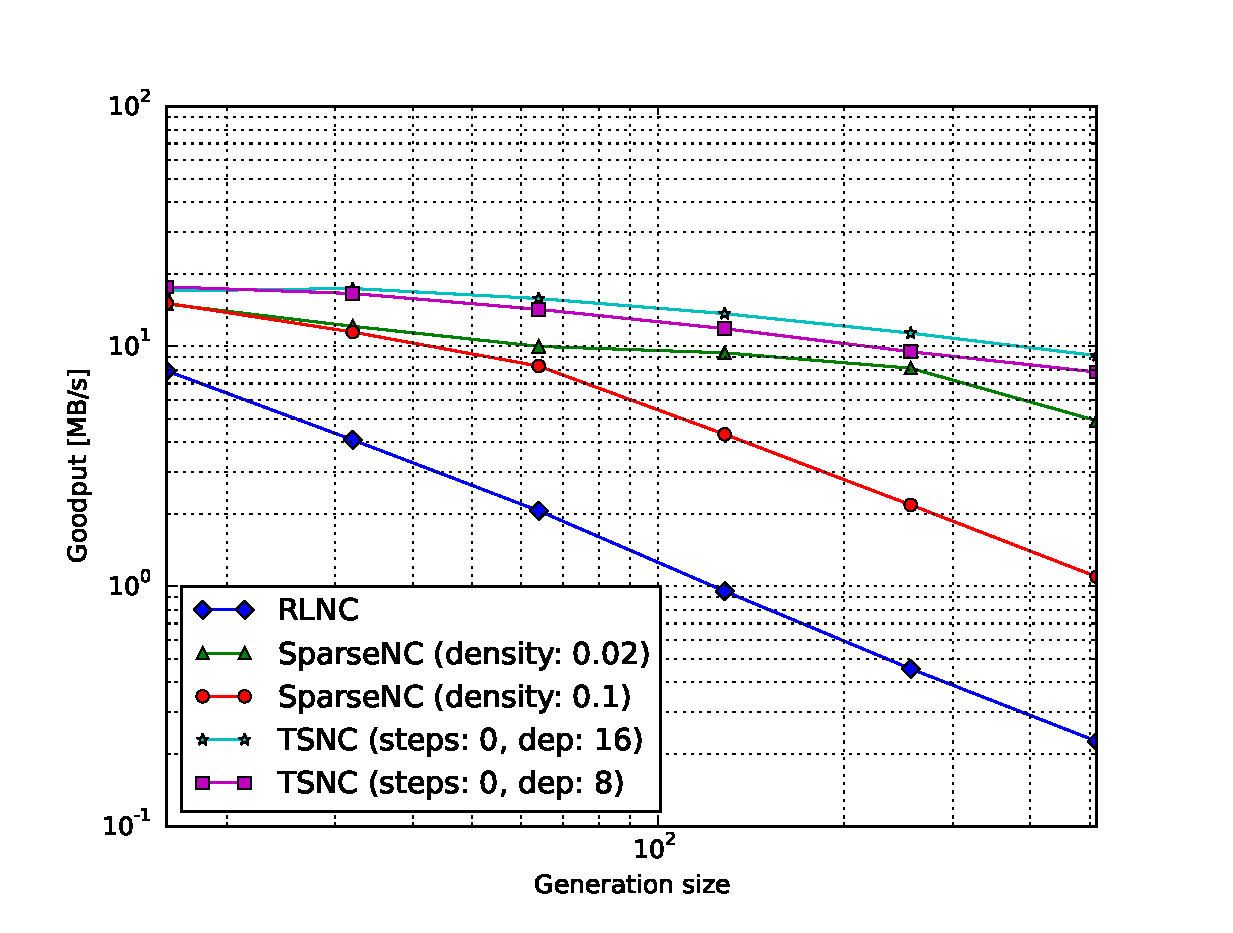
\includegraphics[width=1.15\textwidth]{images/23_07_2015/goodput_vs_generation_size_Rasp_encoder_Binary_1600.eps}
        \caption[]%
        {{\small Goodput vs. Generation size for $q = 2$}}
        \label{fig:enc_good_rasp1_gen_gf2}
    \end{subfigure}
    \hfill
    \begin{subfigure}[b]{0.475\textwidth}
        \centering
        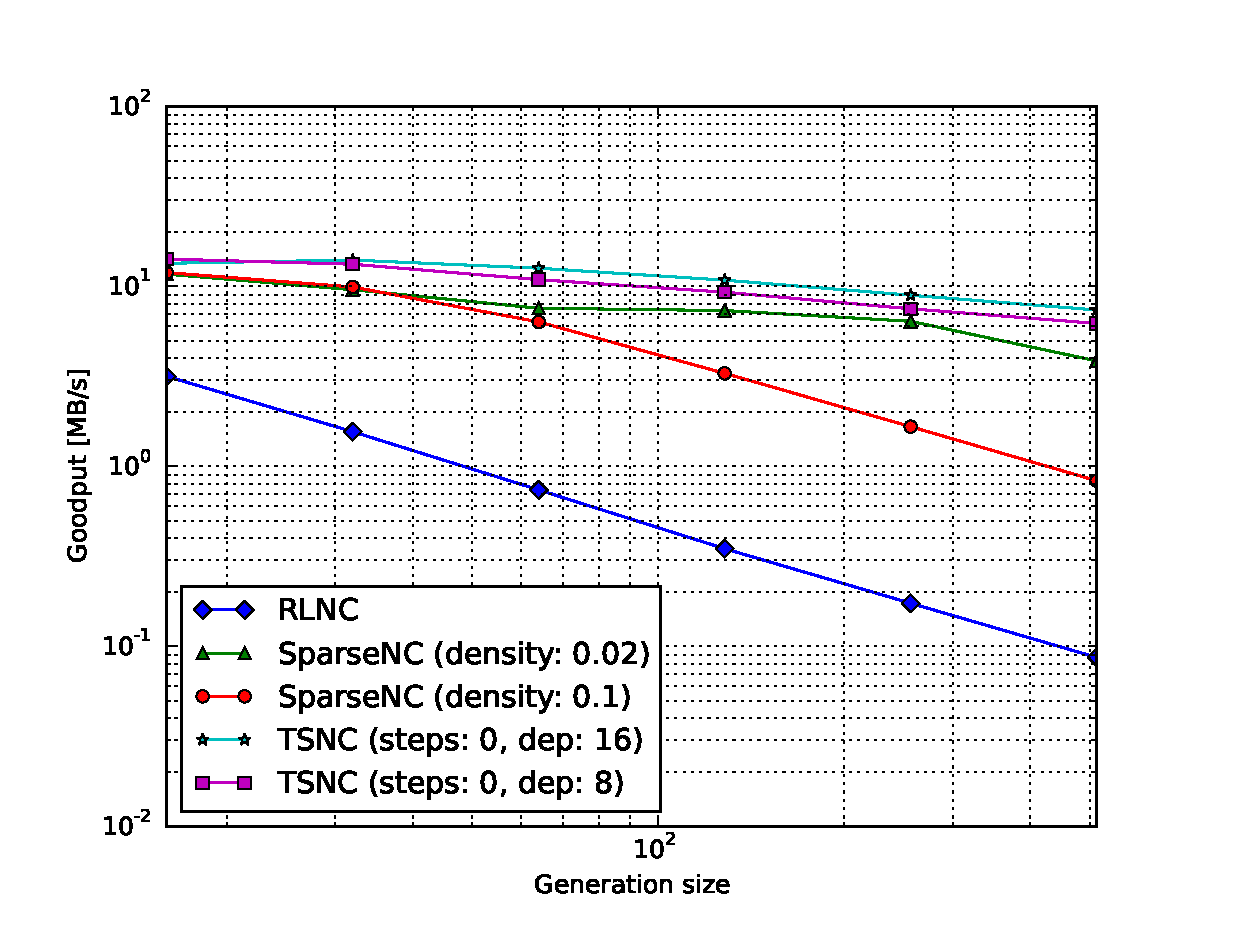
\includegraphics[width=1.15\textwidth]{images/23_07_2015/goodput_vs_generation_size_Rasp_encoder_Binary8_1600.eps}
        \caption[]%
        {{\small Goodput vs. Generation size for $q = 2^8$}}
        \label{fig:enc_good_rasp1_gen_gf256}
    \end{subfigure}
    \vskip\baselineskip
    \begin{subfigure}[b]{0.475\textwidth}
        \centering
        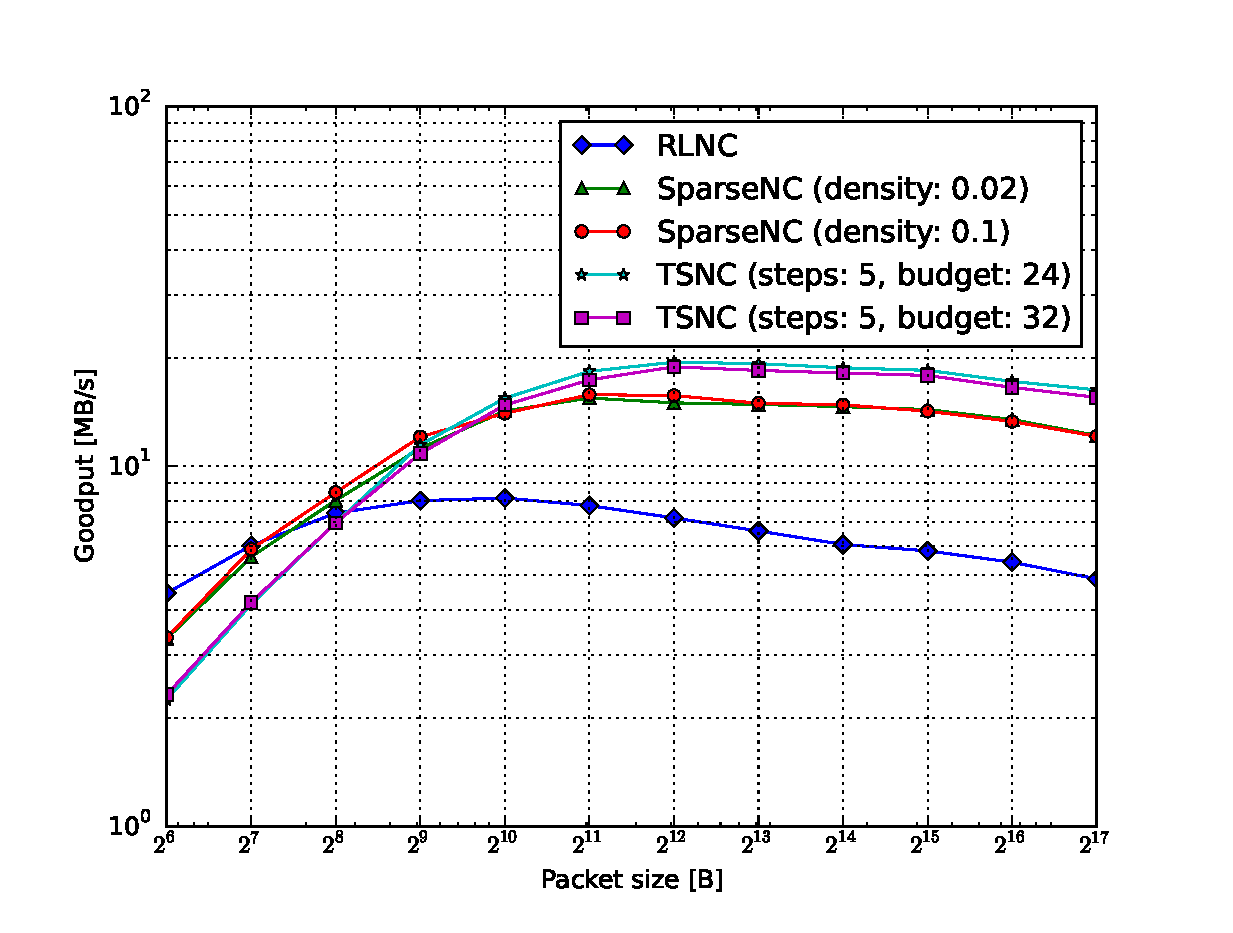
\includegraphics[width=1.15\textwidth]{images/23_07_2015/goodput_vs_symbol_size_Rasp_encoder_Binary_16.eps}
        \caption[]%
        {{\small Goodput vs. Packet size for $q = 2,\ g=16$}}
        \label{fig:enc_good_rasp1_packet_gf2}
    \end{subfigure}
    \quad
    \begin{subfigure}[b]{0.475\textwidth}
        \centering
        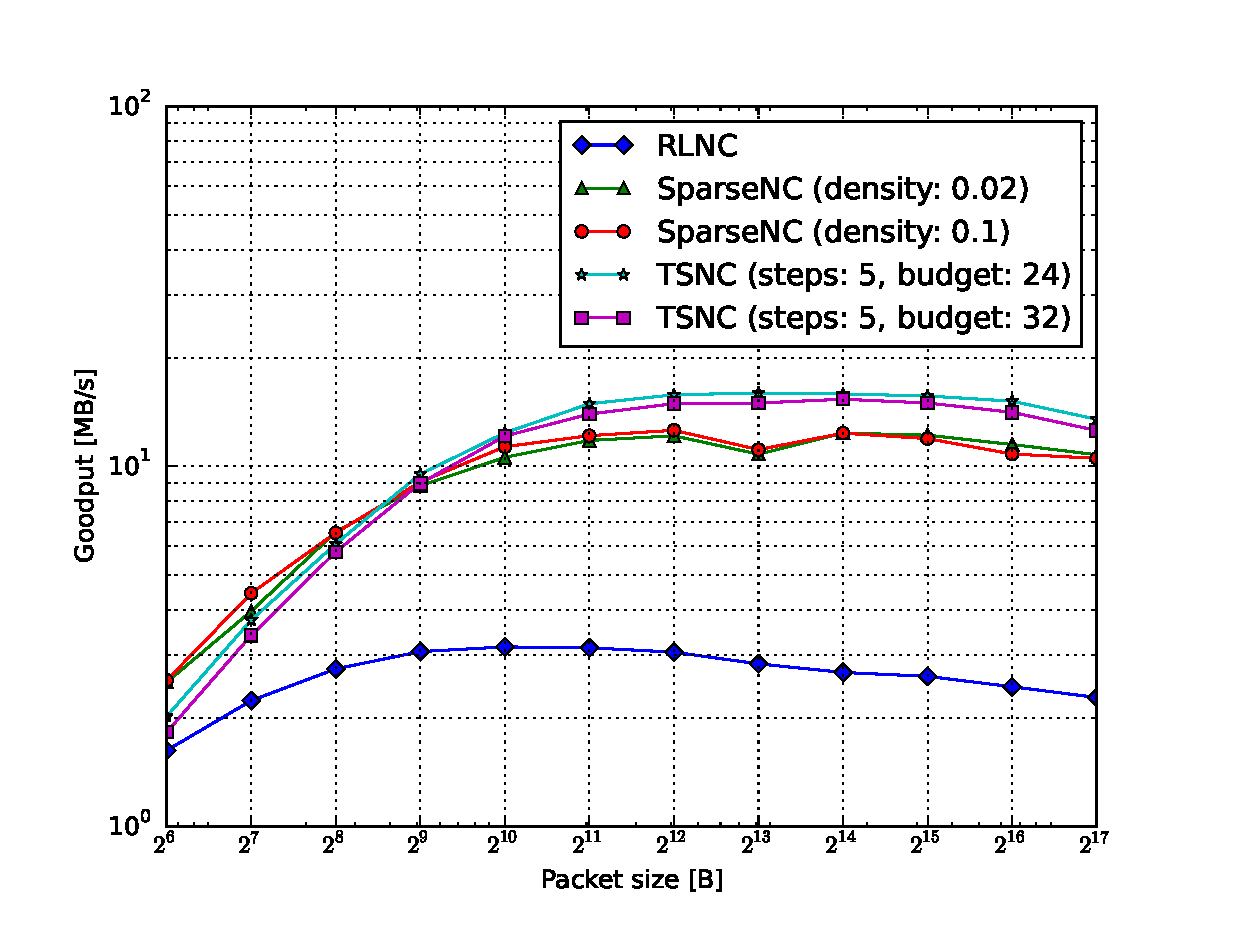
\includegraphics[width=1.15\textwidth]{images/23_07_2015/goodput_vs_symbol_size_Rasp_encoder_Binary8_16.eps}
        \caption[]%
        {{\small Goodput vs. Packet size for $q = 2^8,\ g=16$}}
        \label{fig:enc_good_rasp1_packet_gf256}
    \end{subfigure}
    \caption[]
    {\small Encoder goodput measurements for the \ac{Raspi} 1}
    \label{fig:enc_good_rasp1}
\end{figure*}
%
As it can seen in the from: Figs. \ref{fig:enc_good_rasp1_gen_gf2},
\ref{fig:enc_good_rasp1_gen_gf256}, \ref{fig:enc_good_rasp2_gen_gf2} and
\ref{fig:enc_good_rasp2_gen_gf256}; which indicate the goodput dependency
on the generation size, the encoding goodput gets reduced as the generation
size increases, regardless of the \ac{Raspi} model observed. The reason
is that the encoding operation processing is $\mathcal{O}(g)$ because
it is required to create $g$ coding coefficients and do $g$ multiplications
for each packet. This makes the goodput to scale as the inverse of the
generation size.

In the sets of figures shown in Figs.~\ref{fig:enc_good_rasp1} and
\ref{fig:enc_good_rasp2}, it can be observed that the goodput for $GF(2)$
is higher than for $GF(2^8)$ but still around the same order of magnitud.
This difference is explained by noticing that \ac{GF} arithmetics in the
binary field are simply XOR or AND operations. These operations are
implemented efficiently by most of the architectures nowday and are
tailored to be fast in principle. However, the operations in $GF(2^8)$
are more complex given that the finite field arithmetics have to be
performed with lookup tables which at the end reduces the computing
speed giving a lower goodput when compared with the binary field.

In \ref{fig:enc_good_rasp1_gen_gf2}, \ref{fig:enc_good_rasp1_gen_gf256},
\ref{fig:enc_good_rasp2_gen_gf2} and \ref{fig:enc_good_rasp2_gen_gf256};
it can be seen the goodput trends of 5 codes as a function of
the generation size: \ac{RLNC}, \ac{SRLNC} with $d = [0.02,\ 0.1]$
and \ac{TSNC} with two parameters that we mention. The first of them,
$steps$, is the number of density changes in the system, if any.
The number of changes is equal to the number of regions minus 1, making
$steps = \#regions - 1$ and $dep = e$. With these definitions, we first
evaluate \ac{TSNC} with no changes, e.g. $steps=0$ and the two amounts
for dependent packets mentioned earlier. In this way the budget is
either $g + 8$ or $g + 16$. This means that we tolerate at most 8 or 16
packets regardless of the generation. The goal with setting first
\ac{TSNC} with these values is to observe first the sole effect of the
budget in the code since $steps = 0$ implies no density changes during
the whole process.

For the plots in the mentioned figures from the encoder goodput measurements,
\ac{RLNC} presents the worst performance in terms of goodput and
\ac{TSNC} with $dep = 16$, the best regardless of the \ac{Raspi} model.
Given that the processing time depends in the amount of coded packets
required to create, \ac{RLNC} is the slowest to process since it must
use all of the $g$ original packets. Later, sparse codes process the data
at a larger rate since less packets are being mixed when creating a
coded packet. The caveat of these schemes is that the sparser the code,
the more probable the ocurrences of \ac{l.d.} packets is. So, basically
the sparser the codes, then more overhead due to transmissions of \ac{l.d.}
packets they have since it is more likely to generate the same set of
packets. Excluding the coding coefficients overhead, the overhead due to
transmissions of \ac{l.d.} packets can be very high.
For example, if we consider \ac{TSNC} with $dep=16$ and $g = 16$, the budget
in this case permits to send up to 32 packets which is $2\times$ the generation
size for an overhead of $100\%$ excluding the one from the coding
coefficients. This happens because \ac{TSNC} is allowed to add too much
redundancy in this case, which permits it to use a very low code density $d$.
For \ac{RLNC} this is not the case, since the occurrence of \ac{l.d.} coded
packets is low. Even for $GF(2)$, the average amount of redundancy has proven
to be 1.6 packets after $g$ have been transmitted, much less than the
cases where sparse codes are employed. Overall, we observe that there is
a trade-off between goodput and \ac{l.d.} coded packets transmission
overhead.
%
\begin{figure*}
    \centering
    \begin{subfigure}[b]{0.475\textwidth}
        \centering
        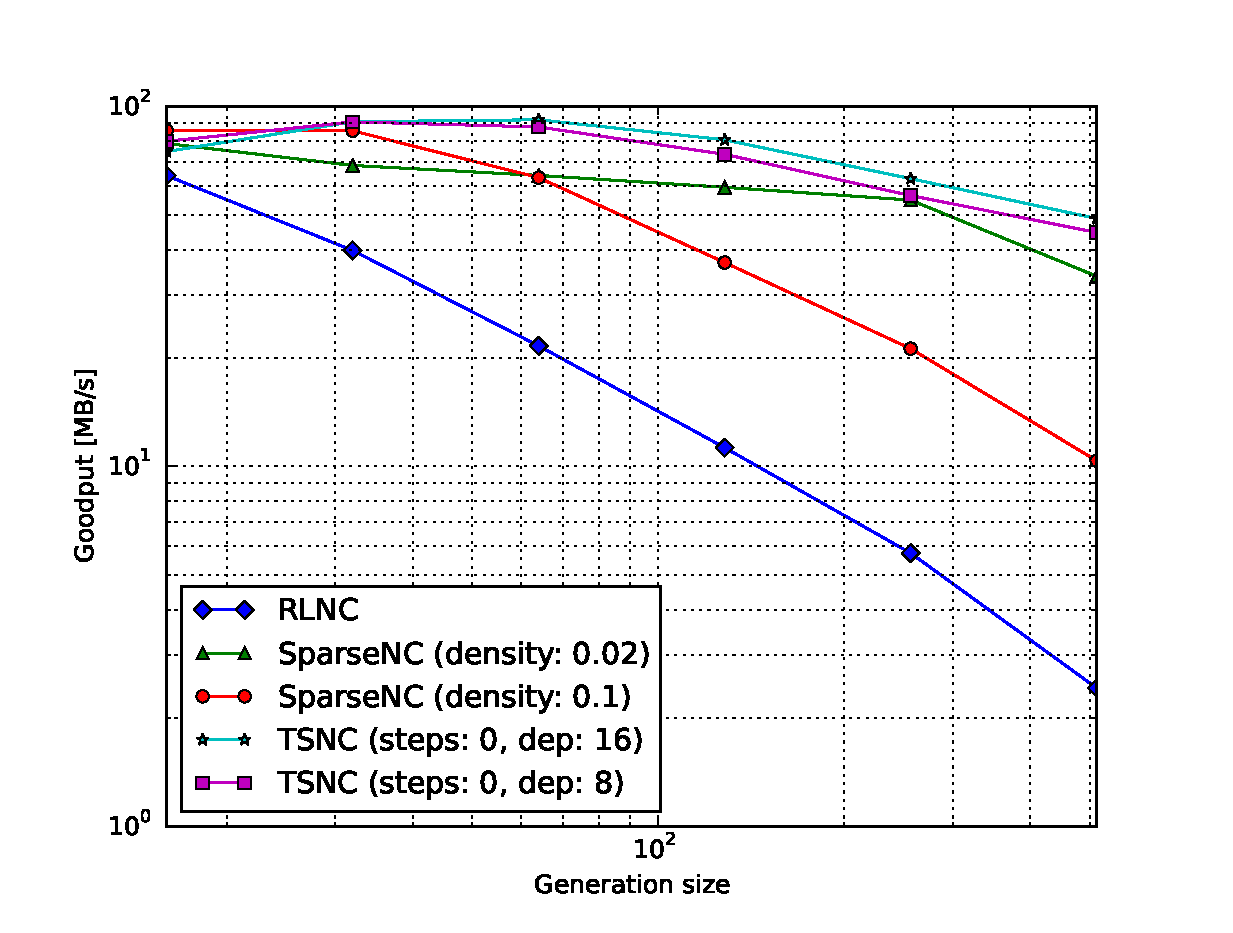
\includegraphics[width=1.15\textwidth]{images/23_07_2015/goodput_vs_generation_size_Rasp_v2_encoder_Binary_1600.eps}
        \caption[]%
        {{\small Goodput vs. Generation size for $q = 2$}}
        \label{fig:enc_good_rasp2_gen_gf2}
    \end{subfigure}
    \hfill
    \begin{subfigure}[b]{0.475\textwidth}
        \centering
        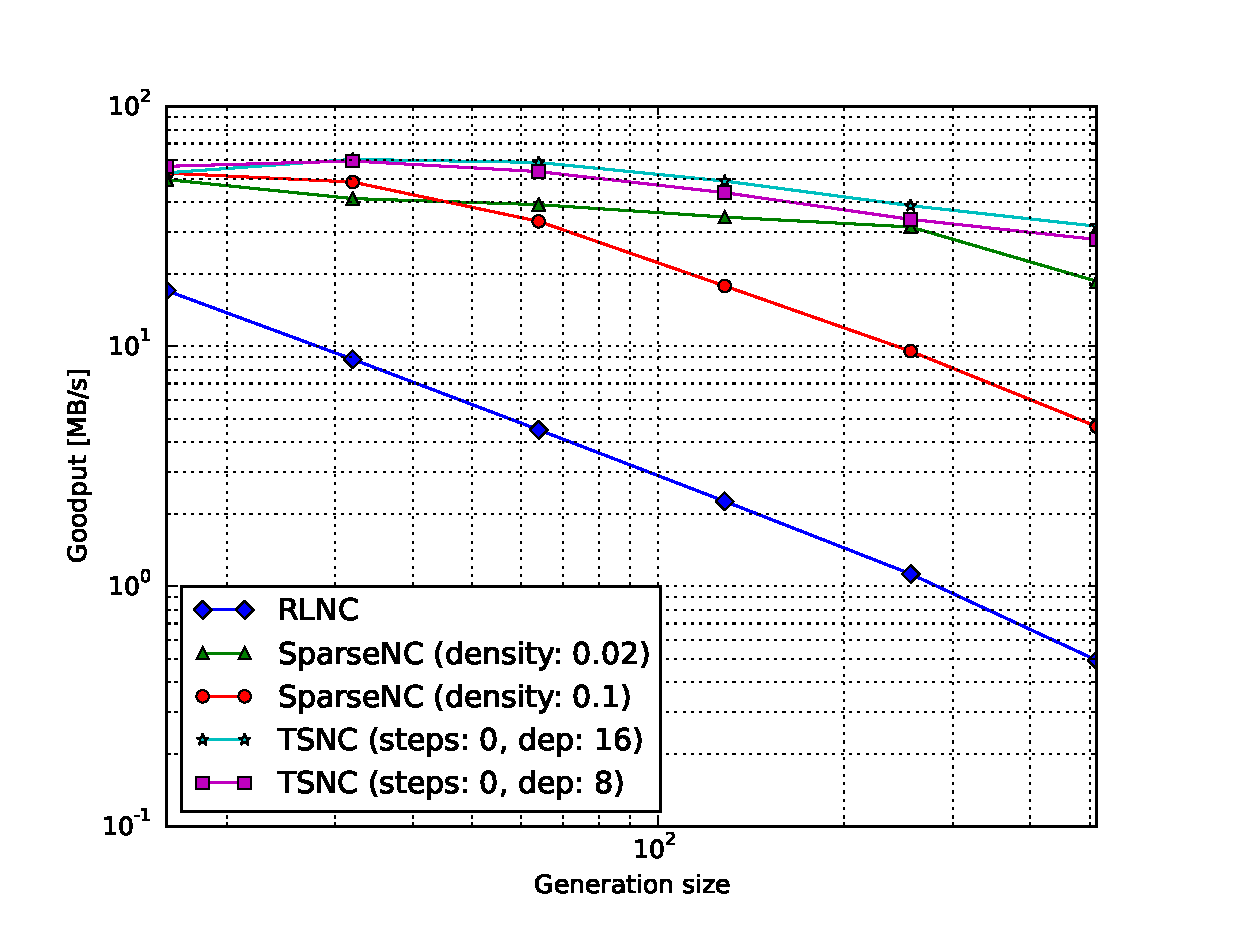
\includegraphics[width=1.15\textwidth]{images/23_07_2015/goodput_vs_generation_size_Rasp_v2_encoder_Binary8_1600.eps}
        \caption[]%
        {{\small Goodput vs. Generation size for $q = 2^8$}}
        \label{fig:enc_good_rasp2_gen_gf256}
    \end{subfigure}
    \vskip\baselineskip
    \begin{subfigure}[b]{0.475\textwidth}
        \centering
        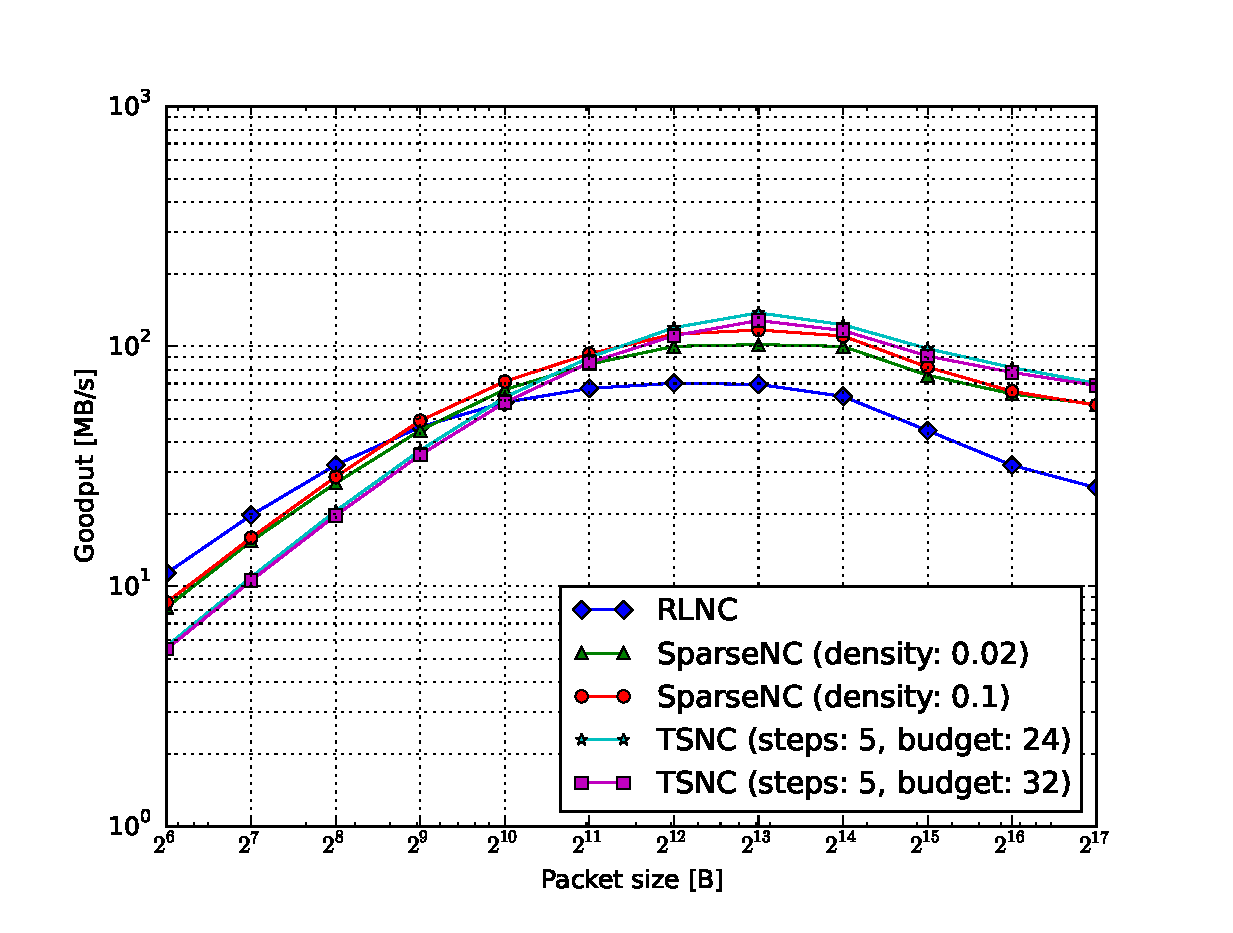
\includegraphics[width=1.15\textwidth]{images/23_07_2015/goodput_vs_symbol_size_Rasp_v2_encoder_Binary_16.eps}
        \caption[]%
        {{\small Goodput vs. Packet size for $q = 2,\ g=16$}}
        \label{fig:enc_good_rasp2_packet_gf2}
    \end{subfigure}
    \quad
    \begin{subfigure}[b]{0.475\textwidth}
        \centering
        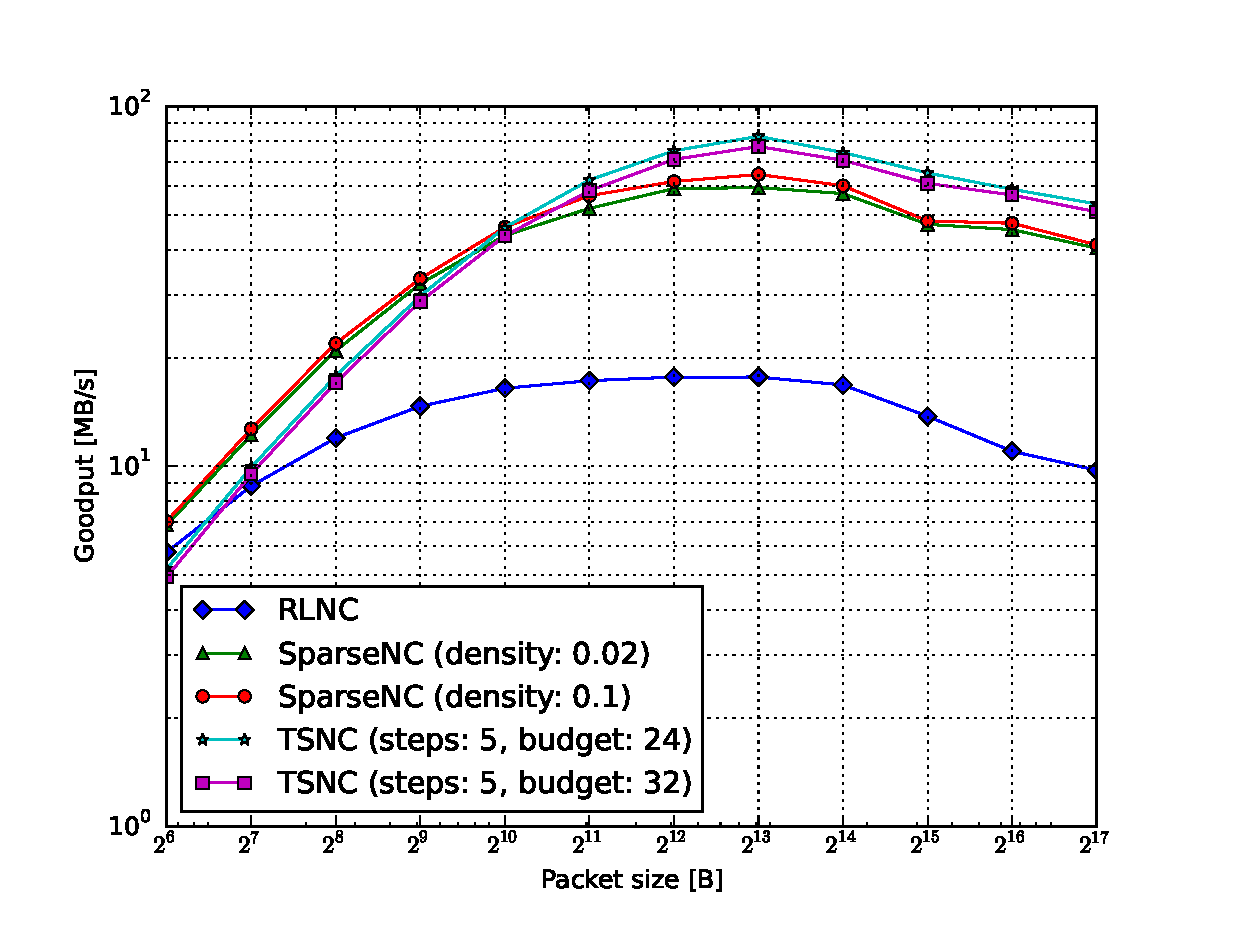
\includegraphics[width=1.15\textwidth]{images/23_07_2015/goodput_vs_symbol_size_Rasp_v2_encoder_Binary8_16.eps}
        \caption[]%
        {{\small Goodput vs. Packet size for $q = 2^8,\ g=16$}}
        \label{fig:enc_good_rasp2_packet_gf256}
    \end{subfigure}
    \caption[]
    {\small Encoder goodput measurements for the \ac{Raspi} 2}
    \label{fig:enc_good_rasp2}
\end{figure*}

Figures description

\subsubsection{Decoding}

We perform the same evaluation as before but now we focus on the decoder.
Fig. \ref{fig:dec_good_rasp1} shows the results of the decoder goodput
measurements for the \ac{Raspi} 1 and Fig. \ref{fig:dec_good_rasp2} does
the proper for \ac{Raspi} 2.

\begin{figure*}
    \centering
    \begin{subfigure}[b]{0.475\textwidth}
        \centering
        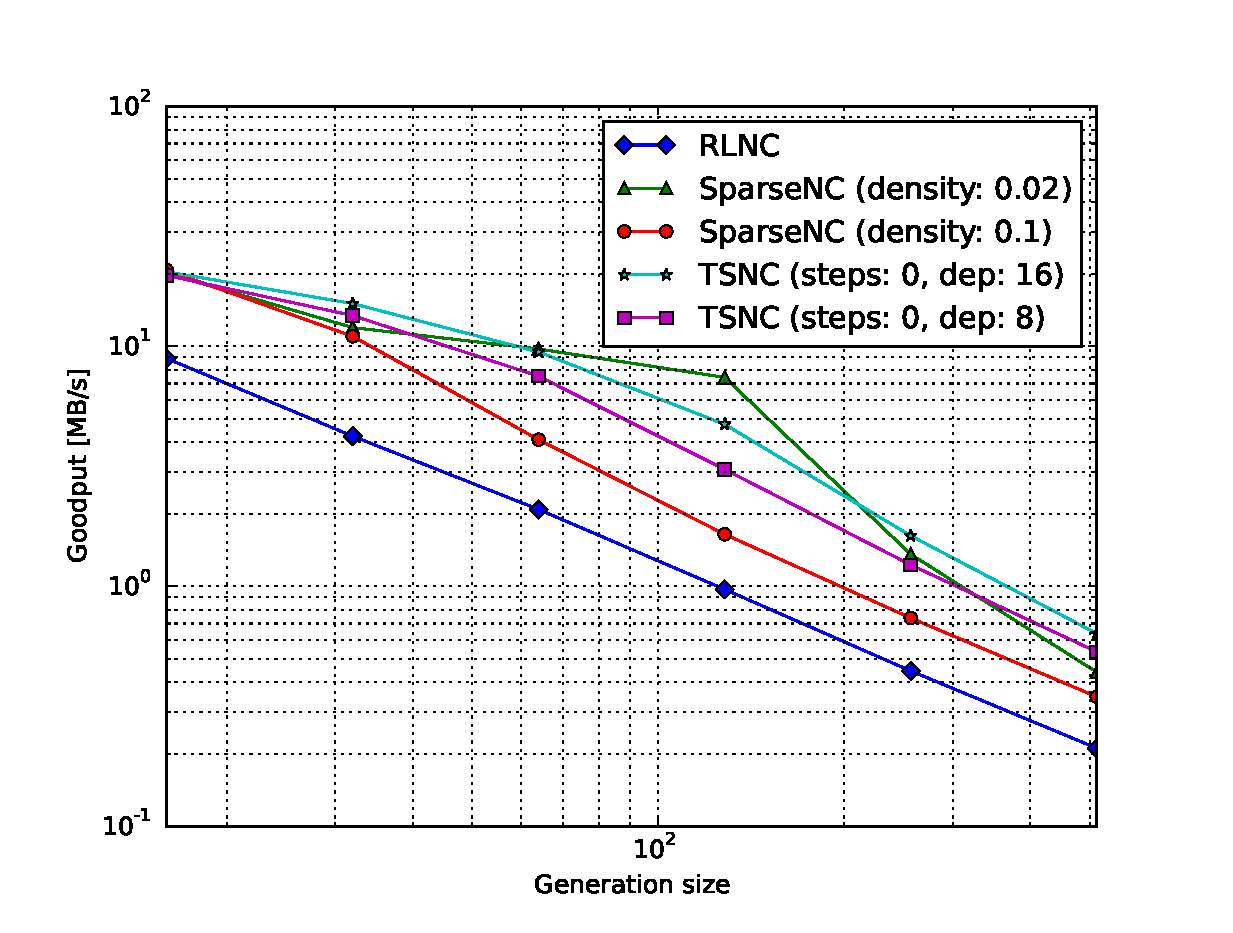
\includegraphics[width=1.15\textwidth]{images/23_07_2015/goodput_vs_generation_size_Rasp_decoder_Binary_1600.eps}
        \caption[]%
        {{\small Goodput vs. Generation size for $q = 2$}}
        \label{fig:dec_good_rasp1_gen_gf2}
    \end{subfigure}
    \hfill
    \begin{subfigure}[b]{0.475\textwidth}
        \centering
        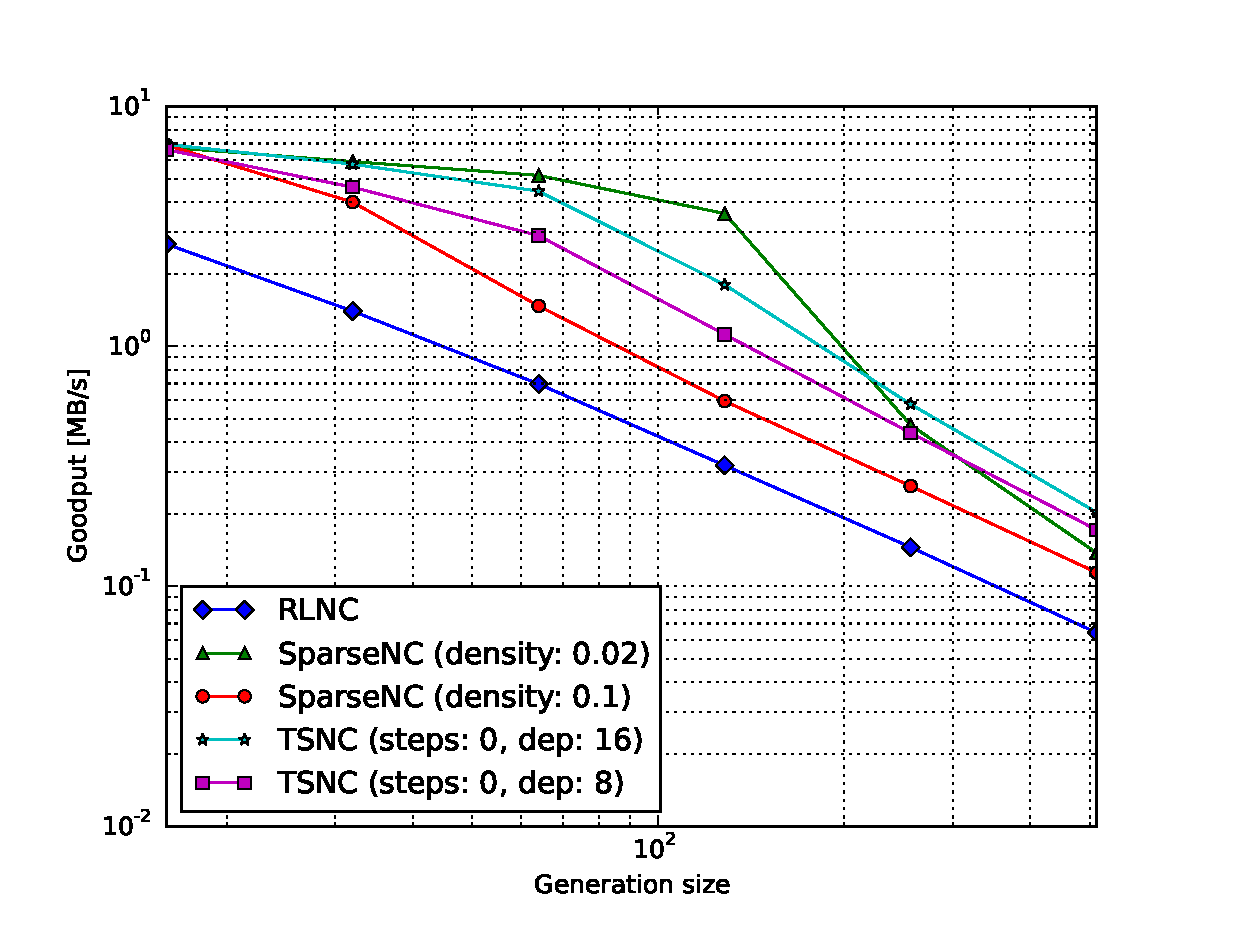
\includegraphics[width=1.15\textwidth]{images/23_07_2015/goodput_vs_generation_size_Rasp_decoder_Binary8_1600.eps}
        \caption[]%
        {{\small Goodput vs. Generation size for $q = 2^8$}}
        \label{fig:dec_good_rasp1_gen_gf256}
    \end{subfigure}
    \vskip\baselineskip
    \begin{subfigure}[b]{0.475\textwidth}
        \centering
        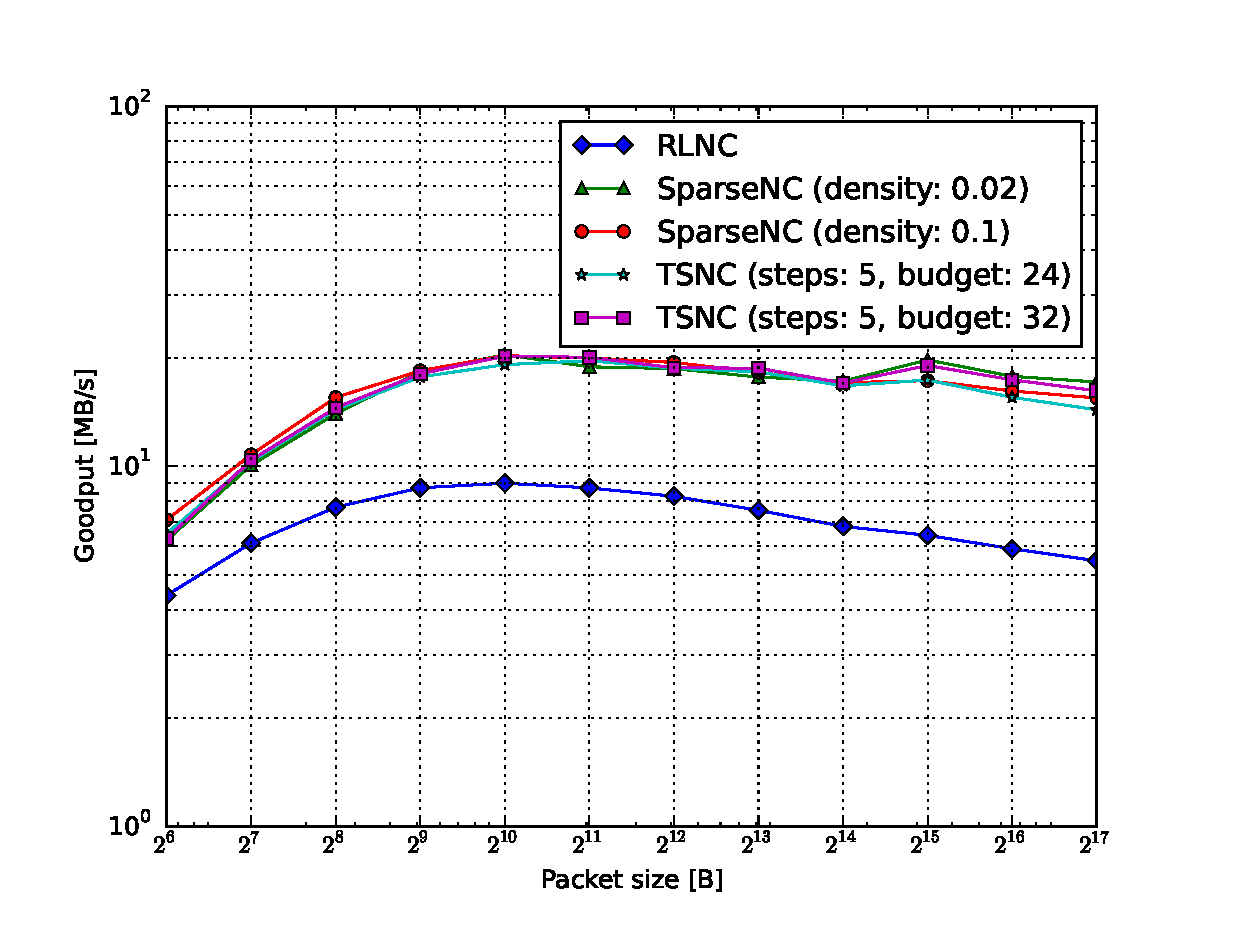
\includegraphics[width=1.15\textwidth]{images/23_07_2015/goodput_vs_symbol_size_Rasp_decoder_Binary_16.eps}
        \caption[]%
        {{\small Goodput vs. Packet size for $q = 2,\ g=16$}}
        \label{fig:dec_good_rasp1_packet_gf2}
    \end{subfigure}
    \quad
    \begin{subfigure}[b]{0.475\textwidth}
        \centering
        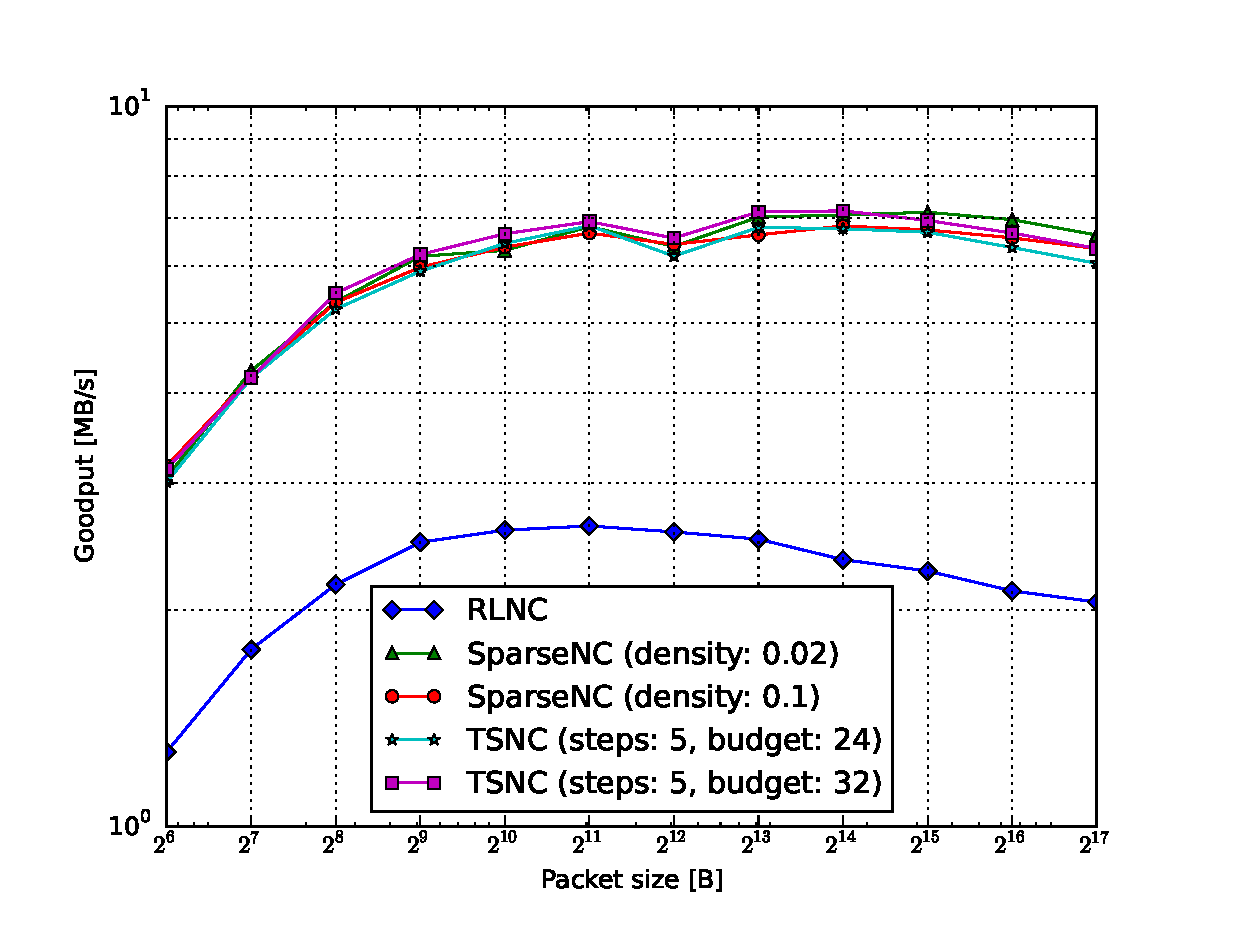
\includegraphics[width=1.15\textwidth]{images/23_07_2015/goodput_vs_symbol_size_Rasp_decoder_Binary8_16.eps}
        \caption[]%
        {{\small Goodput vs. Packet size for $q = 2^8,\ g=16$}}
        \label{fig:dec_good_rasp1_packet_gf256}
    \end{subfigure}
    \caption[]
    {\small Decoder goodput measurements for the \ac{Raspi} 1}
    \label{fig:dec_good_rasp1}
\end{figure*}

Description

\begin{figure*}
    \centering
    \begin{subfigure}[b]{0.475\textwidth}
        \centering
        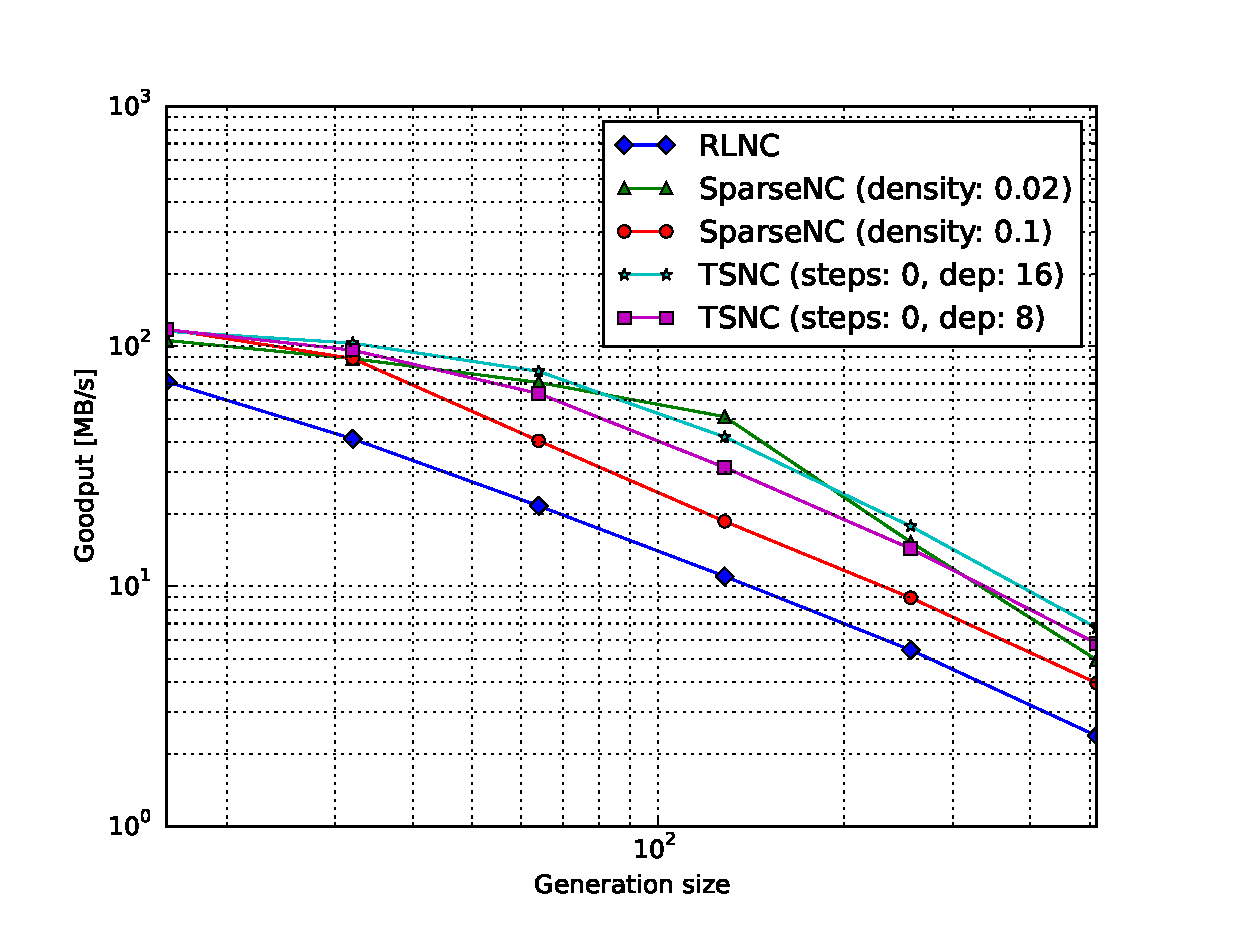
\includegraphics[width=1.15\textwidth]{images/23_07_2015/goodput_vs_generation_size_Rasp_v2_decoder_Binary_1600.eps}
        \caption[]%
        {{\small Goodput vs. Generation size for $q = 2$}}
        \label{fig:dec_good_rasp2_gen_gf2}
    \end{subfigure}
    \hfill
    \begin{subfigure}[b]{0.475\textwidth}
        \centering
        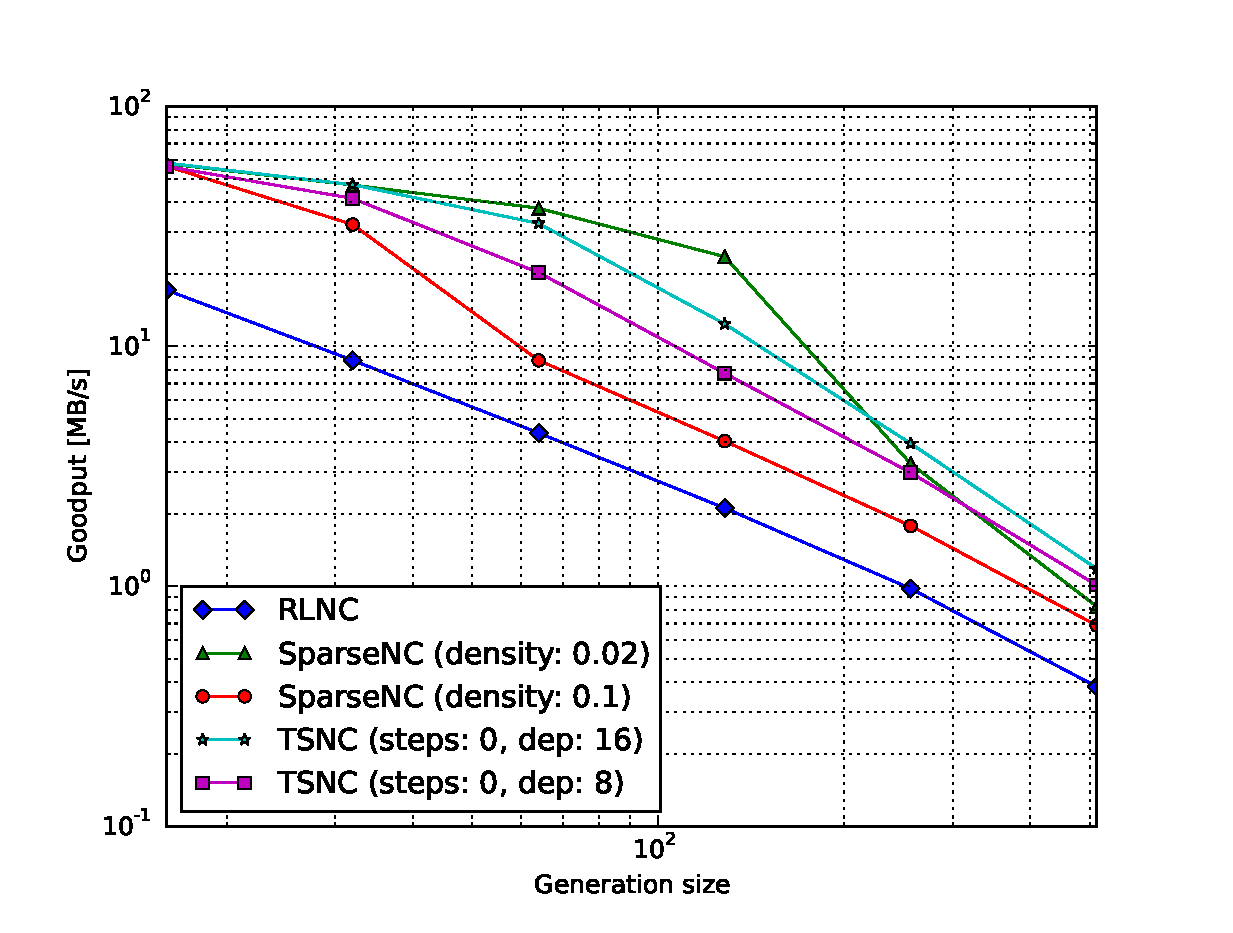
\includegraphics[width=1.15\textwidth]{images/23_07_2015/goodput_vs_generation_size_Rasp_v2_decoder_Binary8_1600.eps}
        \caption[]%
        {{\small Goodput vs. Generation size for $q = 2^8$}}
        \label{fig:dec_good_rasp2_gen_gf256}
    \end{subfigure}
    \vskip\baselineskip
    \begin{subfigure}[b]{0.475\textwidth}
        \centering
        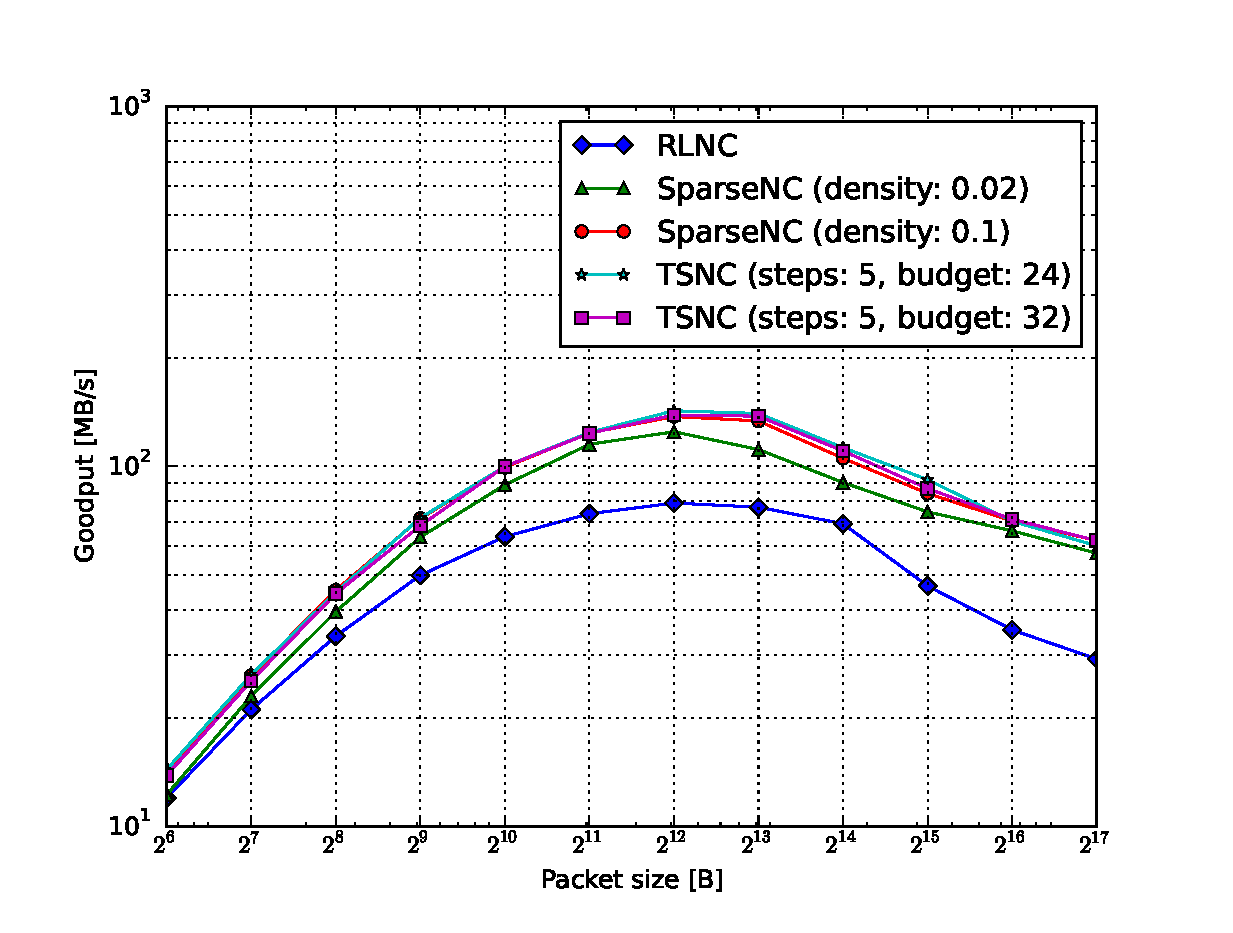
\includegraphics[width=1.15\textwidth]{images/23_07_2015/goodput_vs_symbol_size_Rasp_v2_decoder_Binary_16.eps}
        \caption[]%
        {{\small Goodput vs. Packet size for $q = 2,\ g=16$}}
        \label{fig:dec_good_rasp2_packet_gf2}
    \end{subfigure}
    \quad
    \begin{subfigure}[b]{0.475\textwidth}
        \centering
        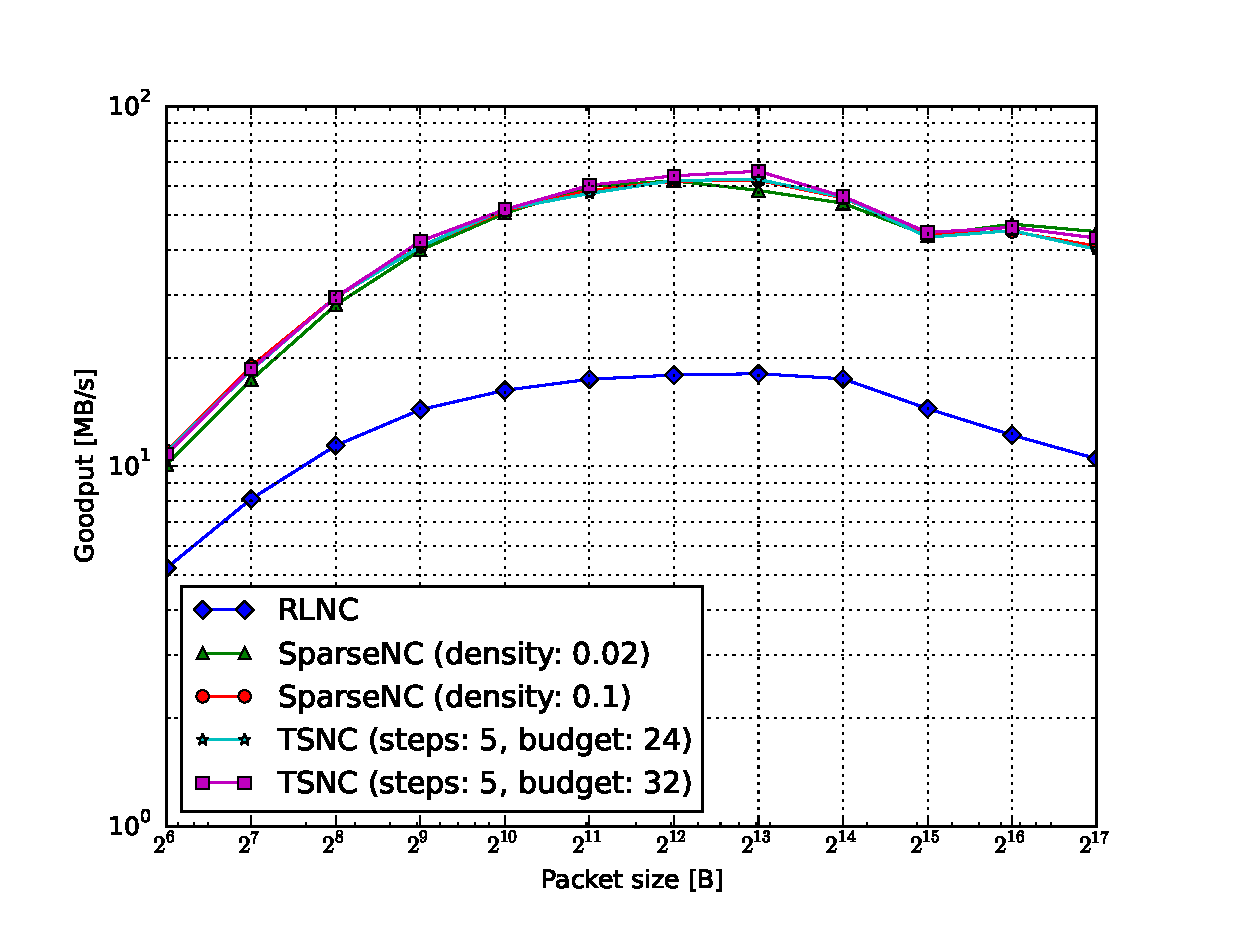
\includegraphics[width=1.15\textwidth]{images/23_07_2015/goodput_vs_symbol_size_Rasp_v2_decoder_Binary8_16.eps}
        \caption[]%
        {{\small Goodput vs. Packet size for $q = 2^8,\ g=16$}}
        \label{fig:dec_good_rasp2_packet_gf256}
    \end{subfigure}
    \caption[]
    {\small Decoder goodput measurements for the \ac{Raspi} 2}
    \label{fig:dec_good_rasp2}
\end{figure*}

Description

\subsection{Average Power}
With the energy measurement setup described in Section \ref{sec:energy_metrics_methods},
we compute the metrics described there. We first proceed with the average
power consumption of the \ac{Raspi} 1 in Fig. \ref{fig:current_rasp1} and
the \ac{Raspi} 2 in Fig. \ref{fig:current_rasp2}.

\begin{figure*}
    \centering
    \begin{subfigure}[b]{0.475\textwidth}
        \centering
        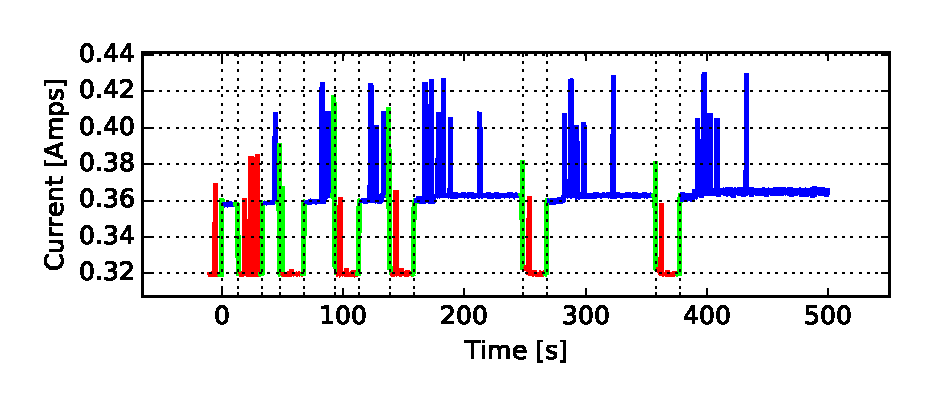
\includegraphics[width=1.15\textwidth]{images/current_vs_sec_raspberry_change_gen_from_-10sec_to_500sec.eps}
        \caption[]%
        {{\small Current for the \ac{Raspi} 1}}
        \label{fig:current_rasp1}
    \end{subfigure}
    \hfill
    \begin{subfigure}[b]{0.475\textwidth}
        \centering
        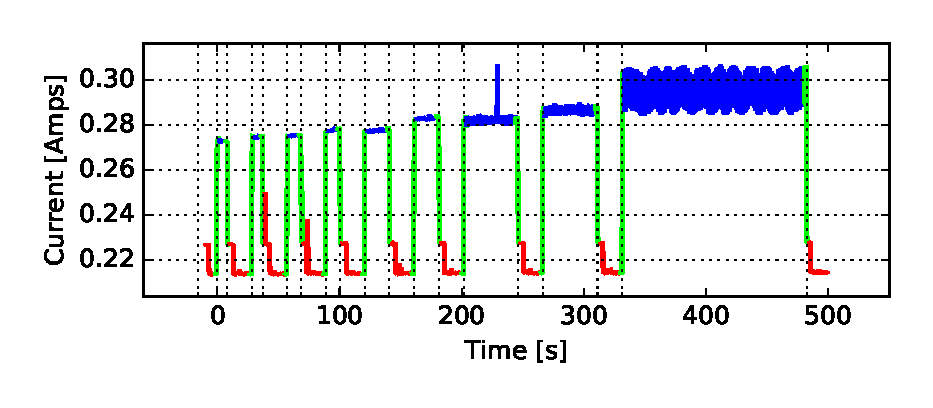
\includegraphics[width=1.15\textwidth]{images/current_vs_sec_raspberry2_change_gen_from_-10sec_to_500sec.eps}
        \caption[]%
        {{\small Current for the \ac{Raspi} 2}}
        \label{fig:current_rasp2}
    \end{subfigure}

    \caption[]
    {\small Current consumption for each \ac{Raspi} model}
    \label{fig:current_rasp}
\end{figure*}

Average current description. Include a table mentioning the current values
and the resulting power values.

\subsection{Energy per bit}
With power and goodput measurements, we compute the energy per bit of
the previously mentioned cases in the same fashion as before.

\subsubsection{Encoding}

\begin{figure*}
    \centering
    \begin{subfigure}[b]{0.475\textwidth}
        \centering
        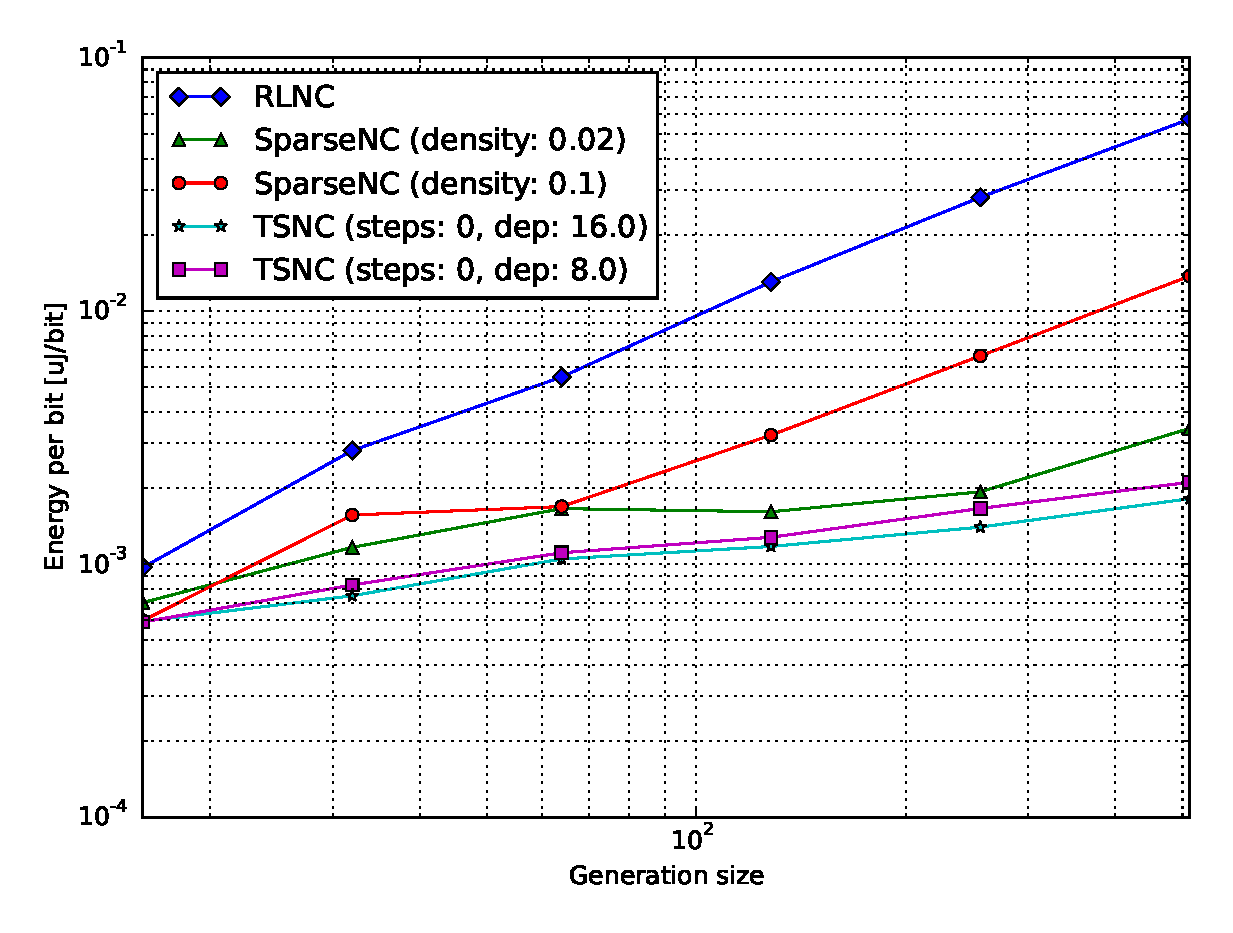
\includegraphics[width=1.1\textwidth]{images/23_07_2015/energy_per_bit_vs_generation_size_Rasp_Binary_encoder_1600.eps}
        \caption[]%
        {{\small Energy per bit vs. Generation size for $q = 2$}}
        \label{fig:enc_ene_rasp1_gen_gf2}
    \end{subfigure}
    \hfill
    \begin{subfigure}[b]{0.475\textwidth}
        \centering
        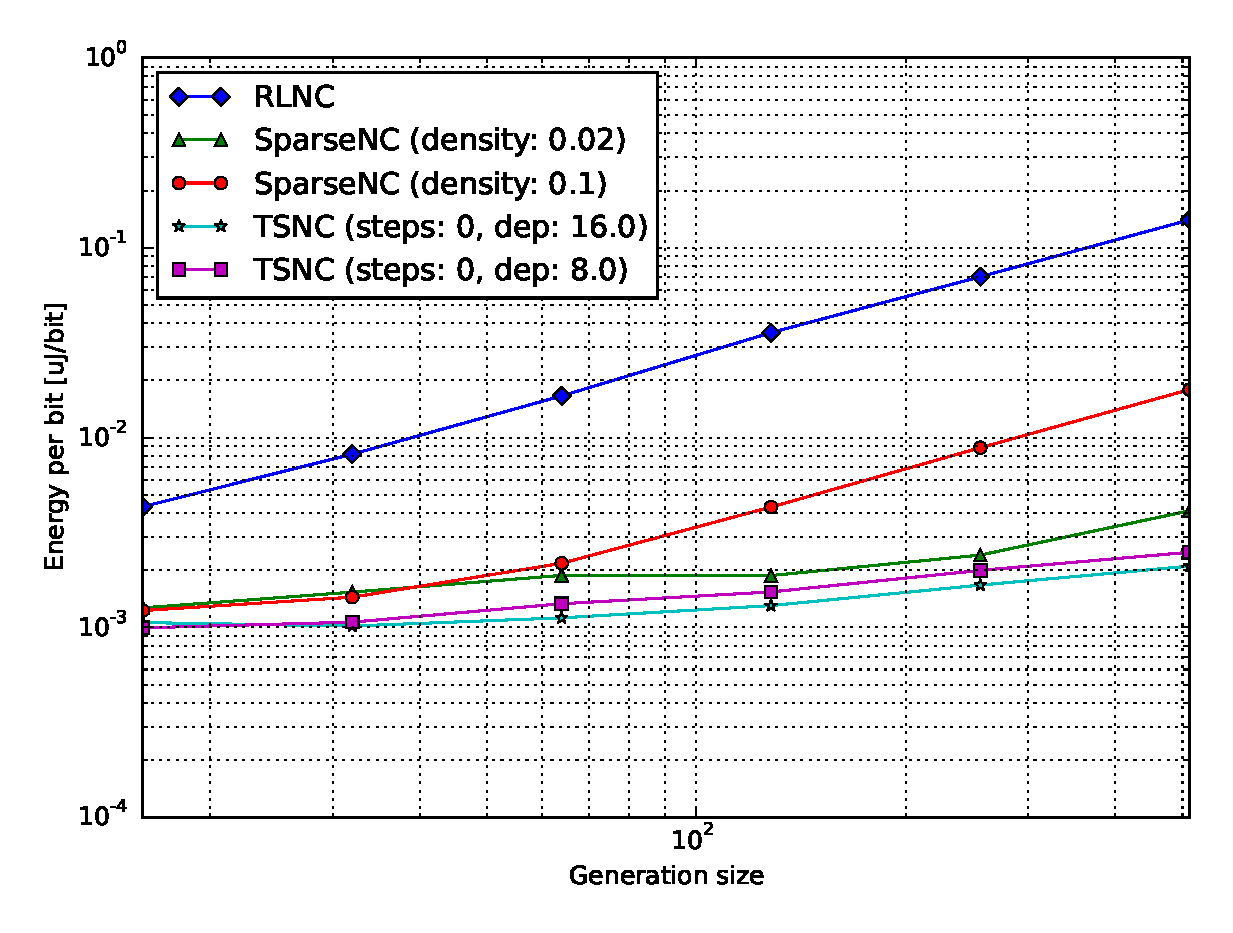
\includegraphics[width=1.1\textwidth]{images/23_07_2015/energy_per_bit_vs_generation_size_Rasp_Binary8_encoder_1600.eps}
        \caption[]%
        {{\small Energy per bit vs. Generation size for $q = 2^8$}}
        \label{fig:enc_ene_rasp1_gen_gf256}
    \end{subfigure}
    \vskip\baselineskip
    \begin{subfigure}[b]{0.475\textwidth}
        \centering
        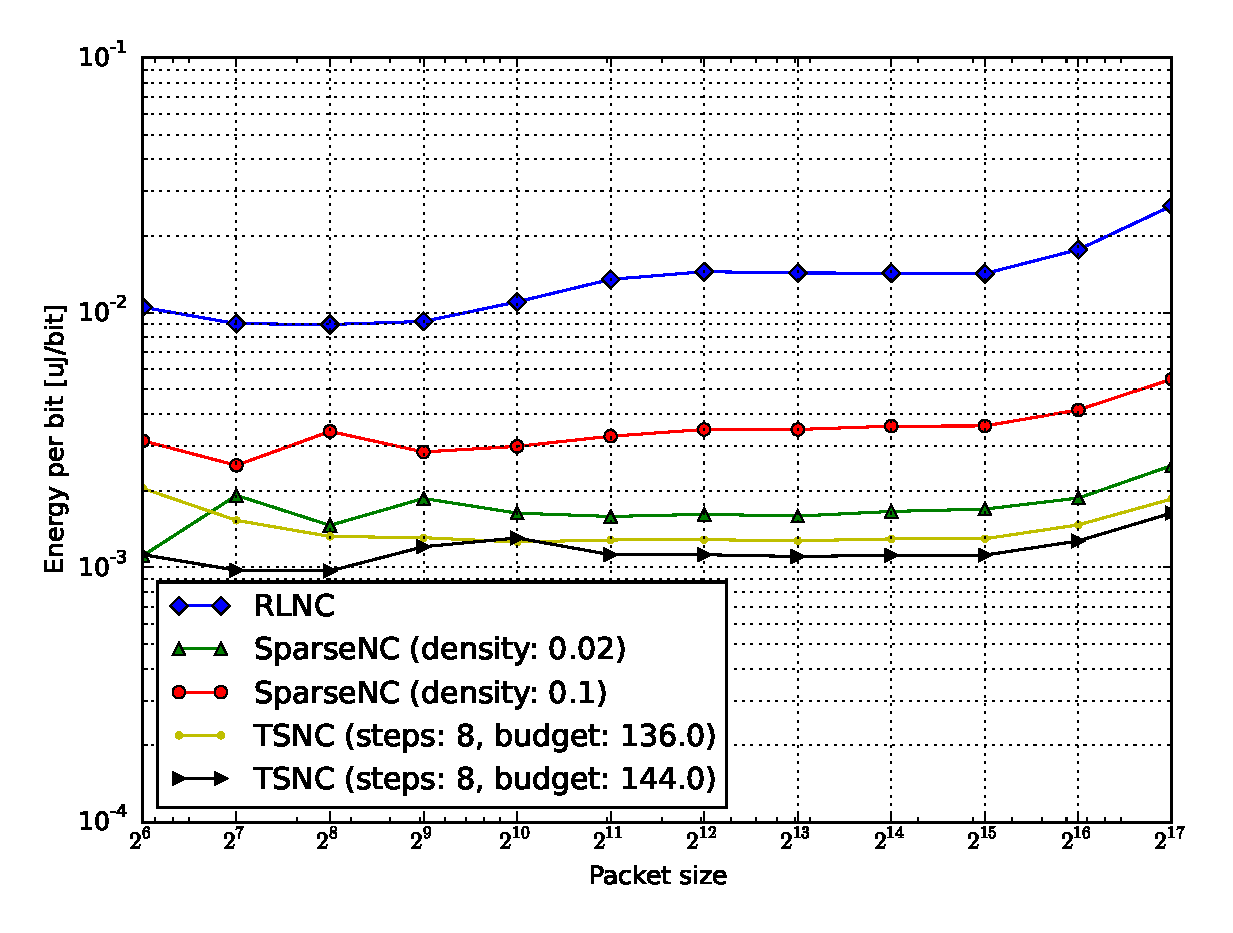
\includegraphics[width=1.1\textwidth]{images/23_07_2015/energy_per_bit_vs_symbol_size_Rasp_Binary_encoder_128.eps}
        \caption[]%
        {{\small Energy per bit vs. Packet size for $q=2,\ g=128$}}
        \label{fig:enc_ene_rasp1_packet_gf2}
    \end{subfigure}
    \quad
    \begin{subfigure}[b]{0.475\textwidth}
        \centering
        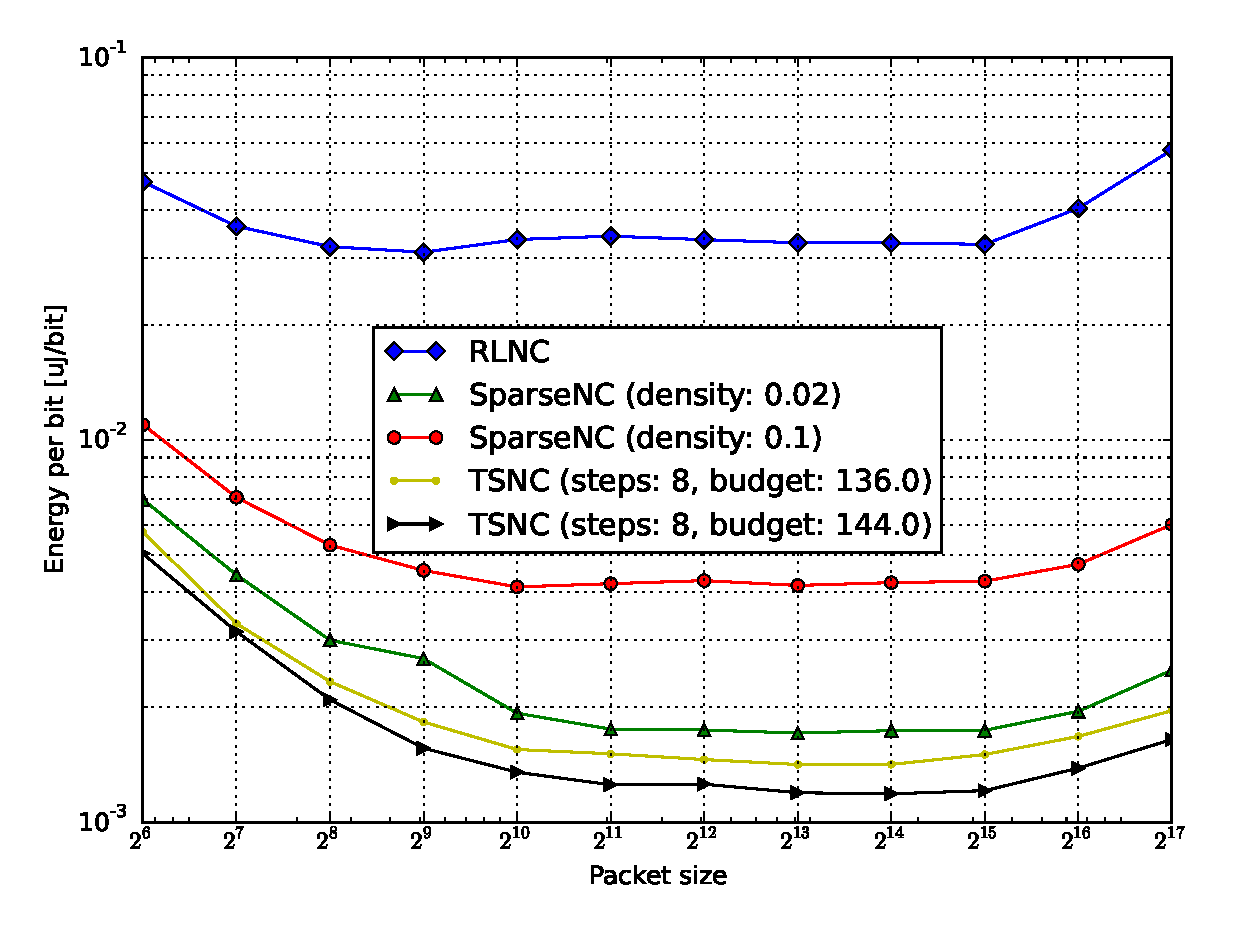
\includegraphics[width=1.1\textwidth]{images/23_07_2015/energy_per_bit_vs_symbol_size_Rasp_Binary8_encoder_128.eps}
        \caption[]%
        {{\small Energy per bit vs. Packet size for $q=2^8,\ g=128$}}
        \label{fig:enc_ene_rasp1_packet_gf256}
    \end{subfigure}
    \caption[]
    {\small Encoder energy measurements for the \ac{Raspi} 1}
    \label{fig:enc_ene_rasp1}
\end{figure*}

Raspi 2 encoding

\begin{figure*}
    \centering
    \begin{subfigure}[b]{0.475\textwidth}
        \centering
        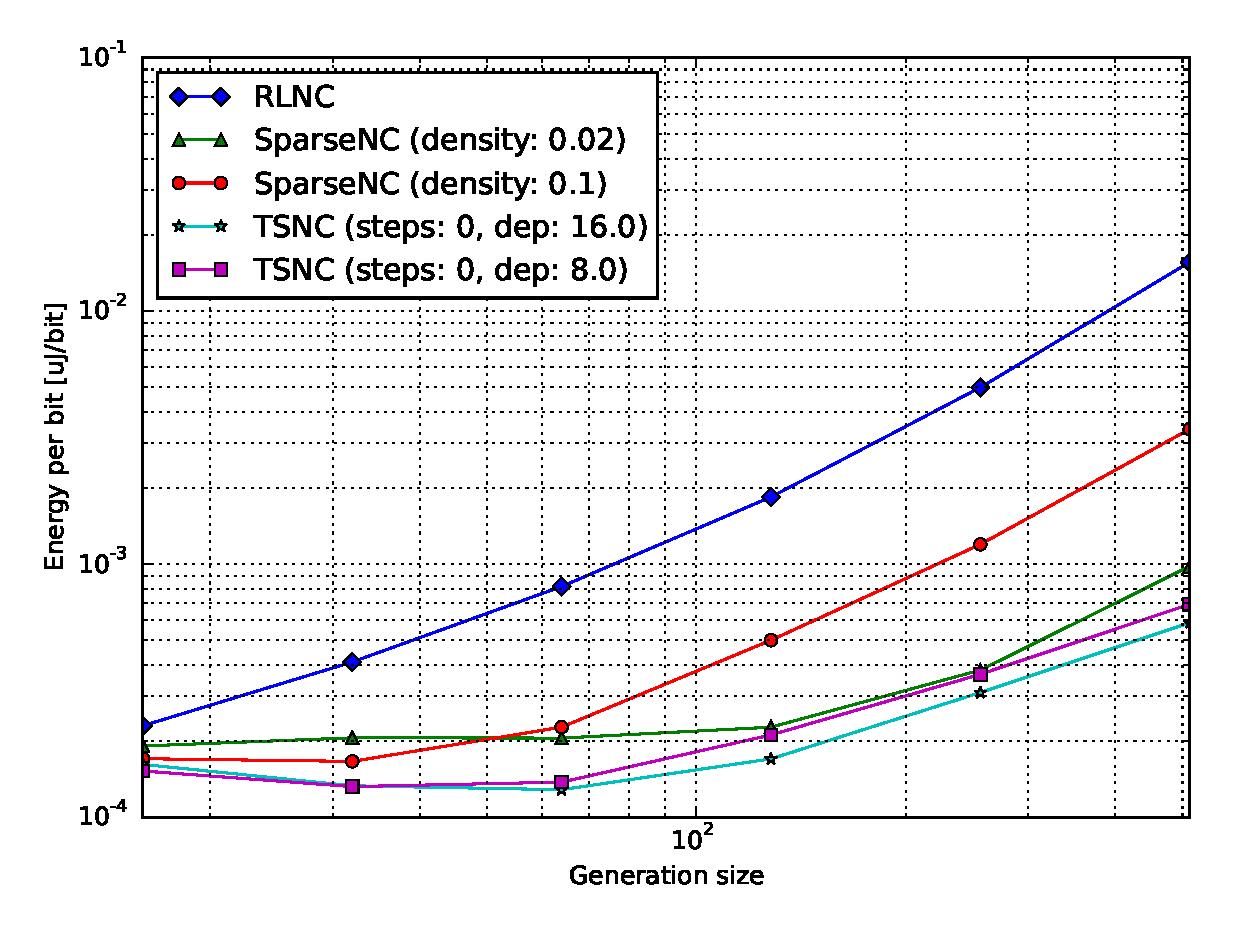
\includegraphics[width=1.1\textwidth]{images/23_07_2015/energy_per_bit_vs_generation_size_Rasp_v2_Binary_encoder_1600.eps}
        \caption[]%
        {{\small Energy per bit vs. Generation size for $q = 2$}}
        \label{fig:enc_ene_rasp2_gen_gf2}
    \end{subfigure}
    \hfill
    \begin{subfigure}[b]{0.475\textwidth}
        \centering
        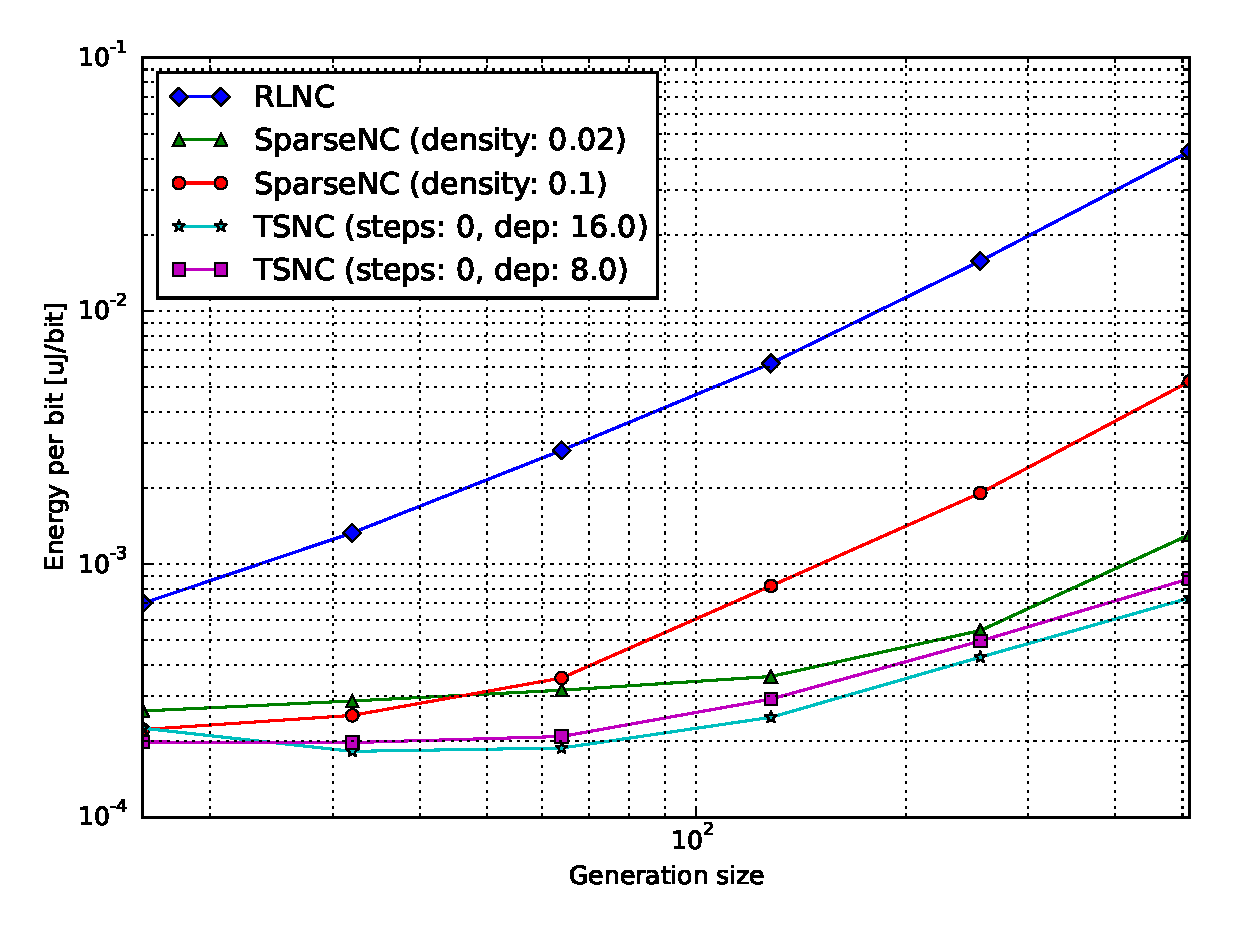
\includegraphics[width=1.1\textwidth]{images/23_07_2015/energy_per_bit_vs_generation_size_Rasp_v2_Binary8_encoder_1600.eps}
        \caption[]%
        {{\small Energy per bit vs. Generation size for $q = 2^8$}}
        \label{fig:enc_ene_rasp2_gen_gf256}
    \end{subfigure}
    \vskip\baselineskip
    \begin{subfigure}[b]{0.475\textwidth}
        \centering
        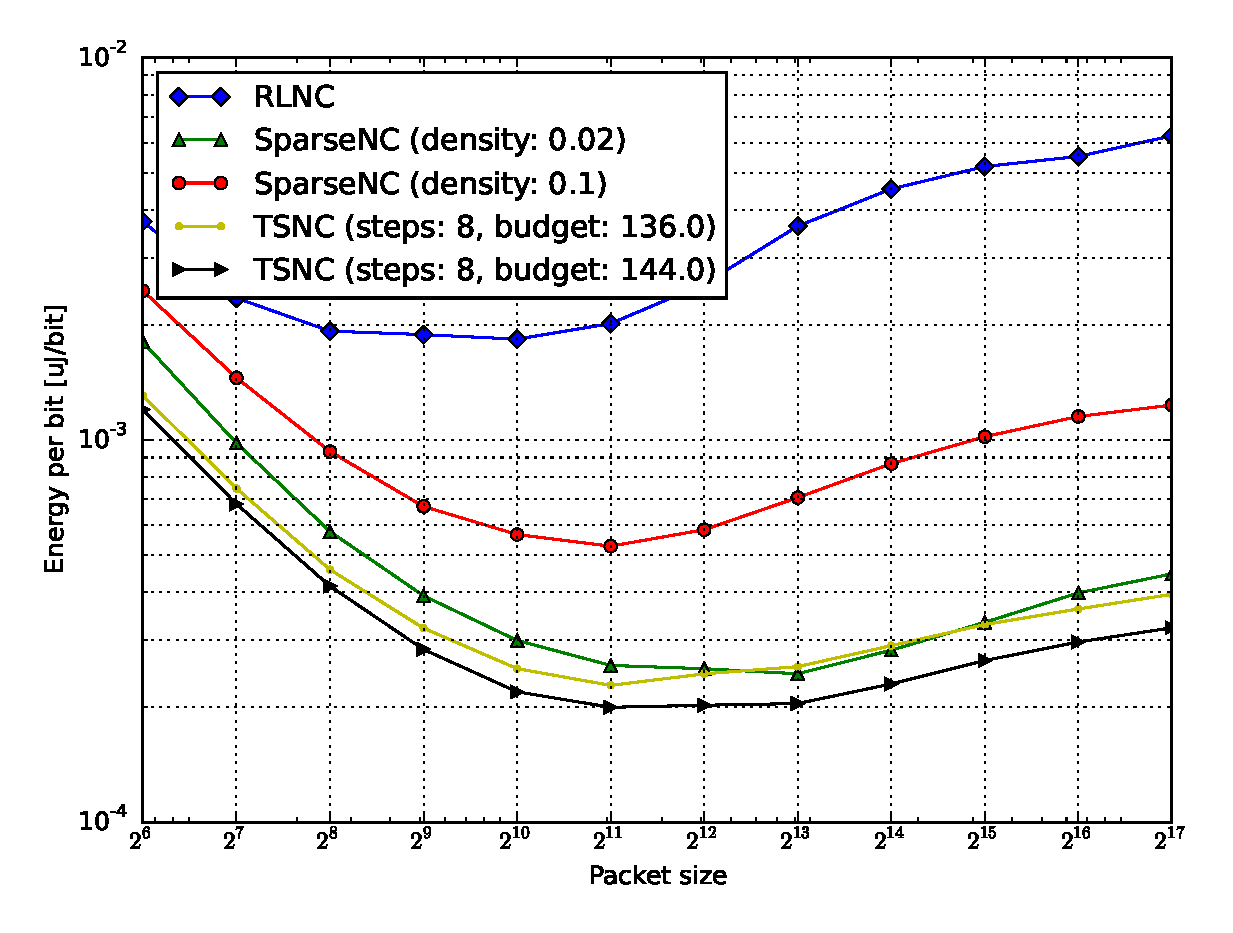
\includegraphics[width=1.1\textwidth]{images/23_07_2015/energy_per_bit_vs_symbol_size_Rasp_v2_Binary_encoder_128.eps}
        \caption[]%
        {{\small Energy per bit vs. Packet size for $q=2,\ g=128$}}
        \label{fig:enc_ene_rasp2_packet_gf2}
    \end{subfigure}
    \quad
    \begin{subfigure}[b]{0.475\textwidth}
        \centering
        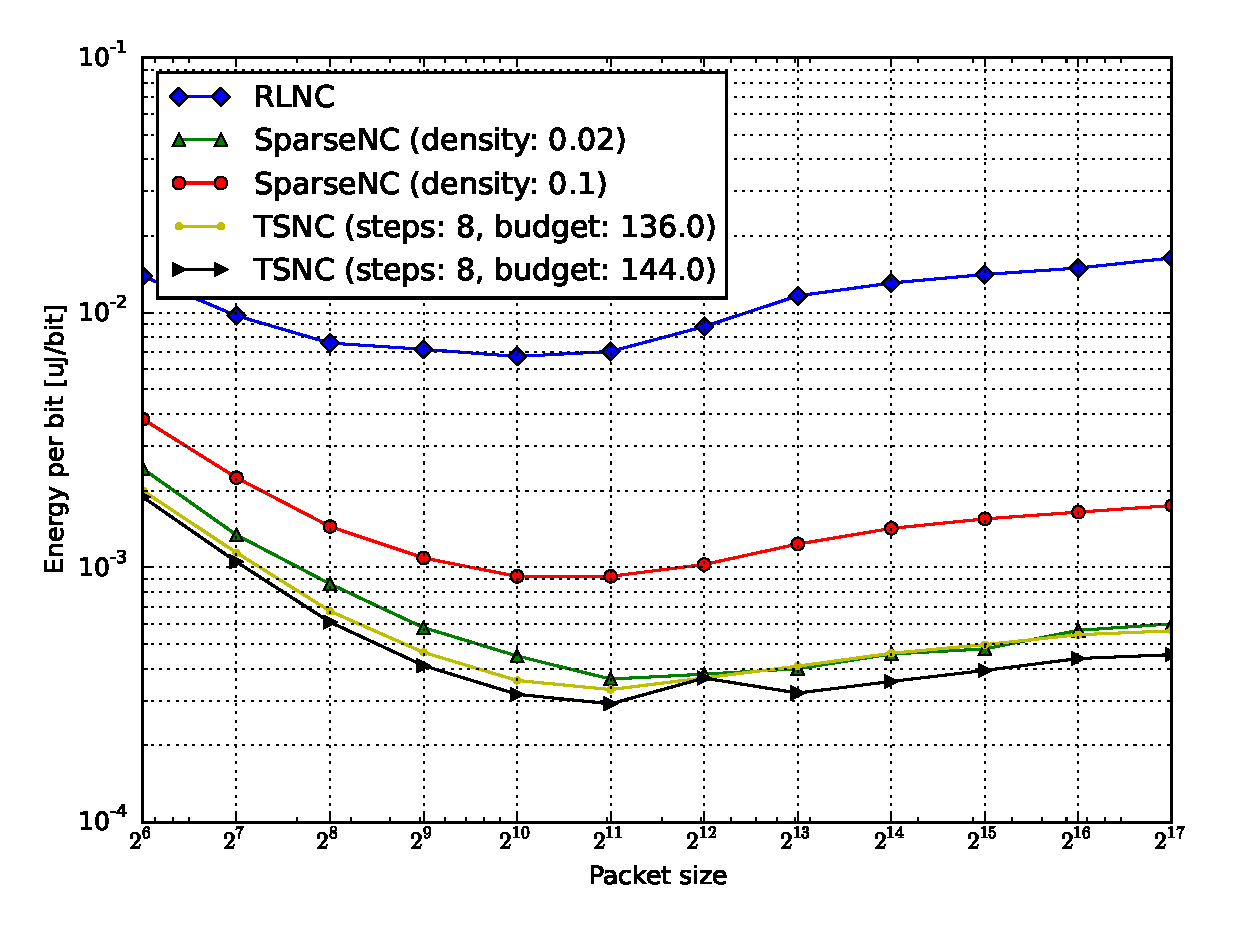
\includegraphics[width=1.1\textwidth]{images/23_07_2015/energy_per_bit_vs_symbol_size_Rasp_v2_Binary8_encoder_128.eps}
        \caption[]%
        {{\small Energy per bit vs. Packet size for $q=2^8,\ g=128$}}
        \label{fig:enc_ene_rasp2_packet_gf256}
    \end{subfigure}
    \caption[]
    {\small Encoder energy measurements for the \ac{Raspi} 2}
    \label{fig:enc_ene_rasp2}
\end{figure*}

\subsubsection{Decoding}

\begin{figure*}
    \centering
    \begin{subfigure}[b]{0.475\textwidth}
        \centering
        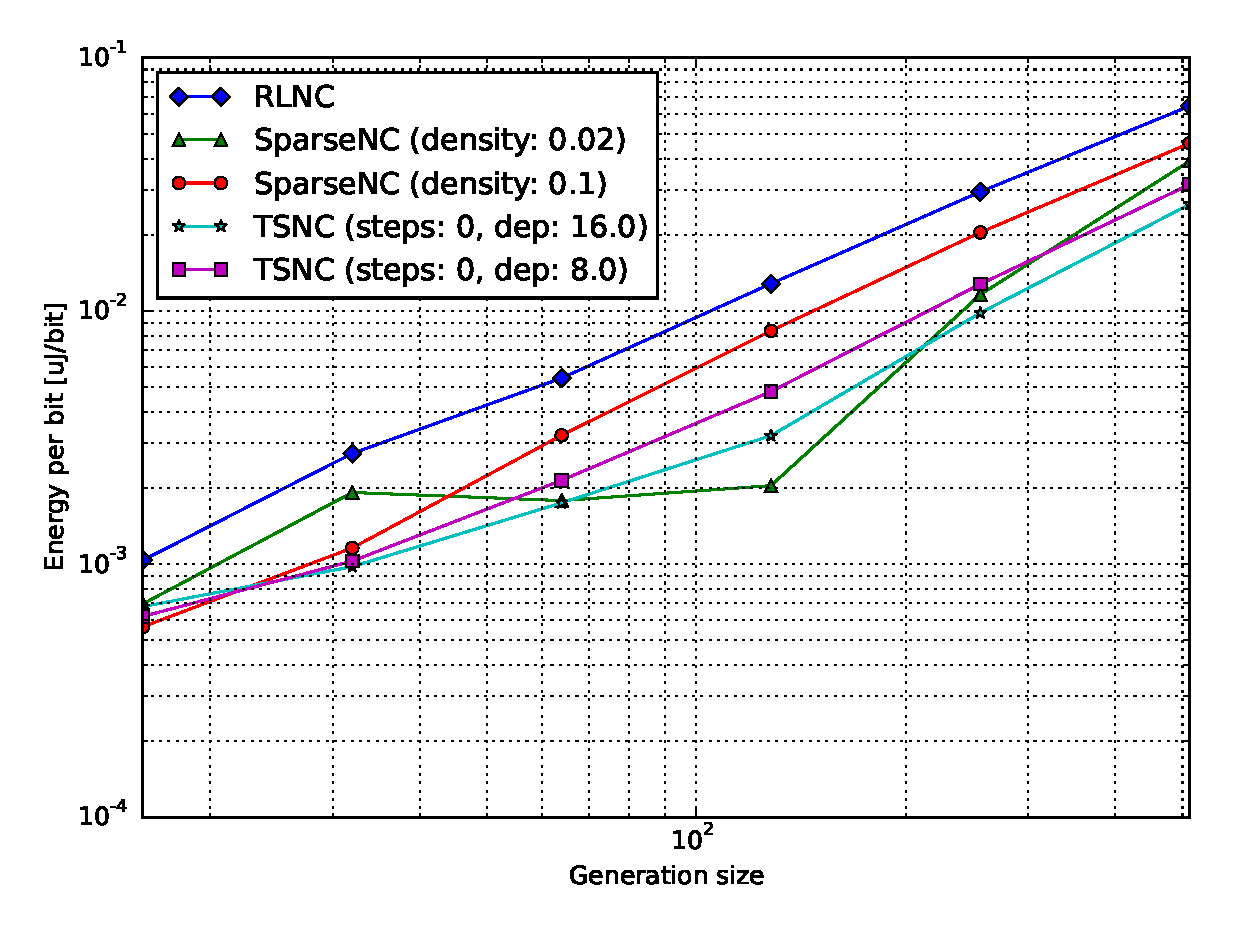
\includegraphics[width=1.1\textwidth]{images/23_07_2015/energy_per_bit_vs_generation_size_Rasp_Binary_decoder_1600.eps}
        \caption[]%
        {{\small Energy per bit vs. Generation size for $q = 2$}}
        \label{fig:dec_ene_rasp1_gen_gf2}
    \end{subfigure}
    \hfill
    \begin{subfigure}[b]{0.475\textwidth}
        \centering
        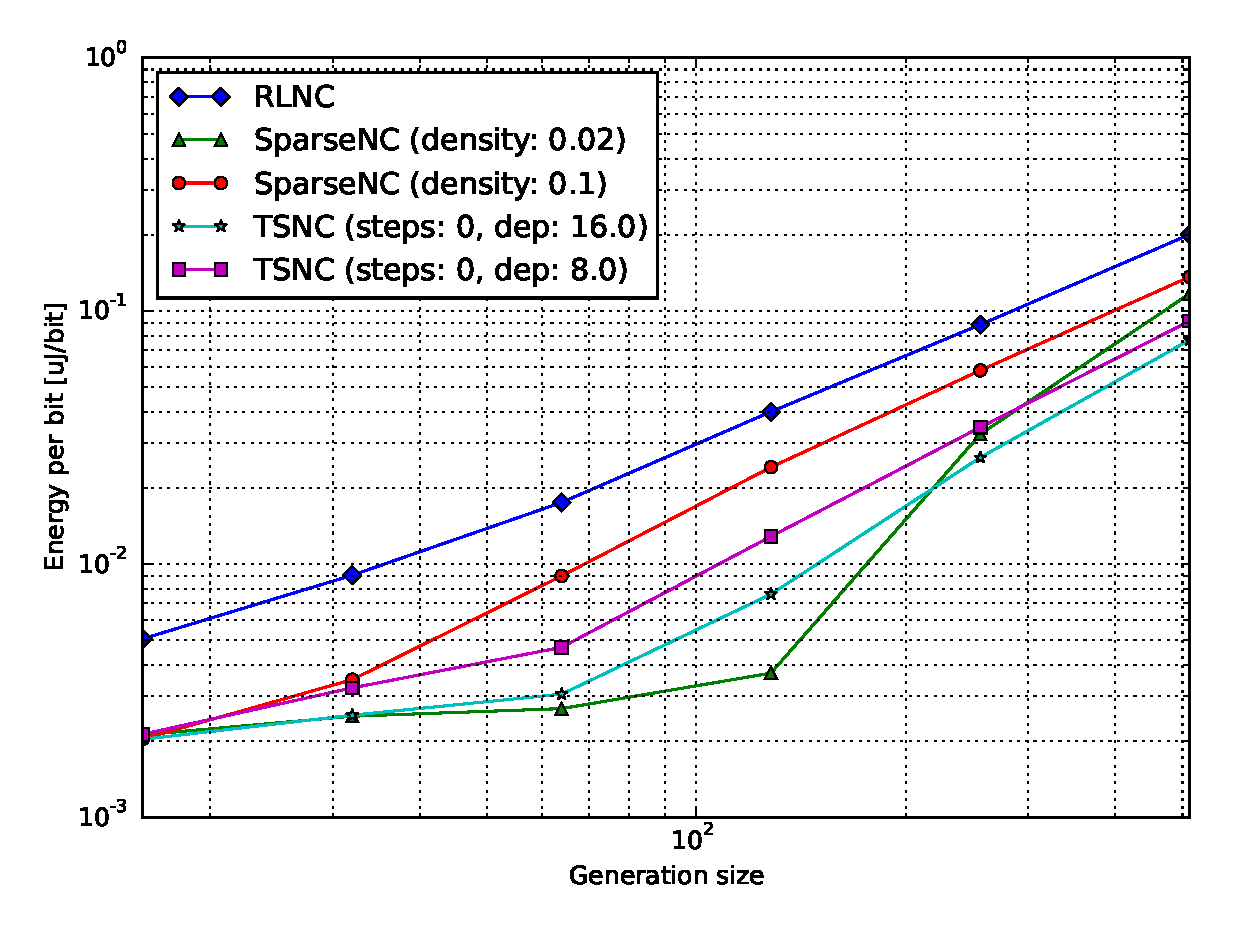
\includegraphics[width=1.1\textwidth]{images/23_07_2015/energy_per_bit_vs_generation_size_Rasp_Binary8_decoder_1600.eps}
        \caption[]%
        {{\small Energy per bit vs. Generation size for $q = 2^8$}}
        \label{fig:dec_ene_rasp1_gen_gf256}
    \end{subfigure}
    \vskip\baselineskip
    \begin{subfigure}[b]{0.475\textwidth}
        \centering
        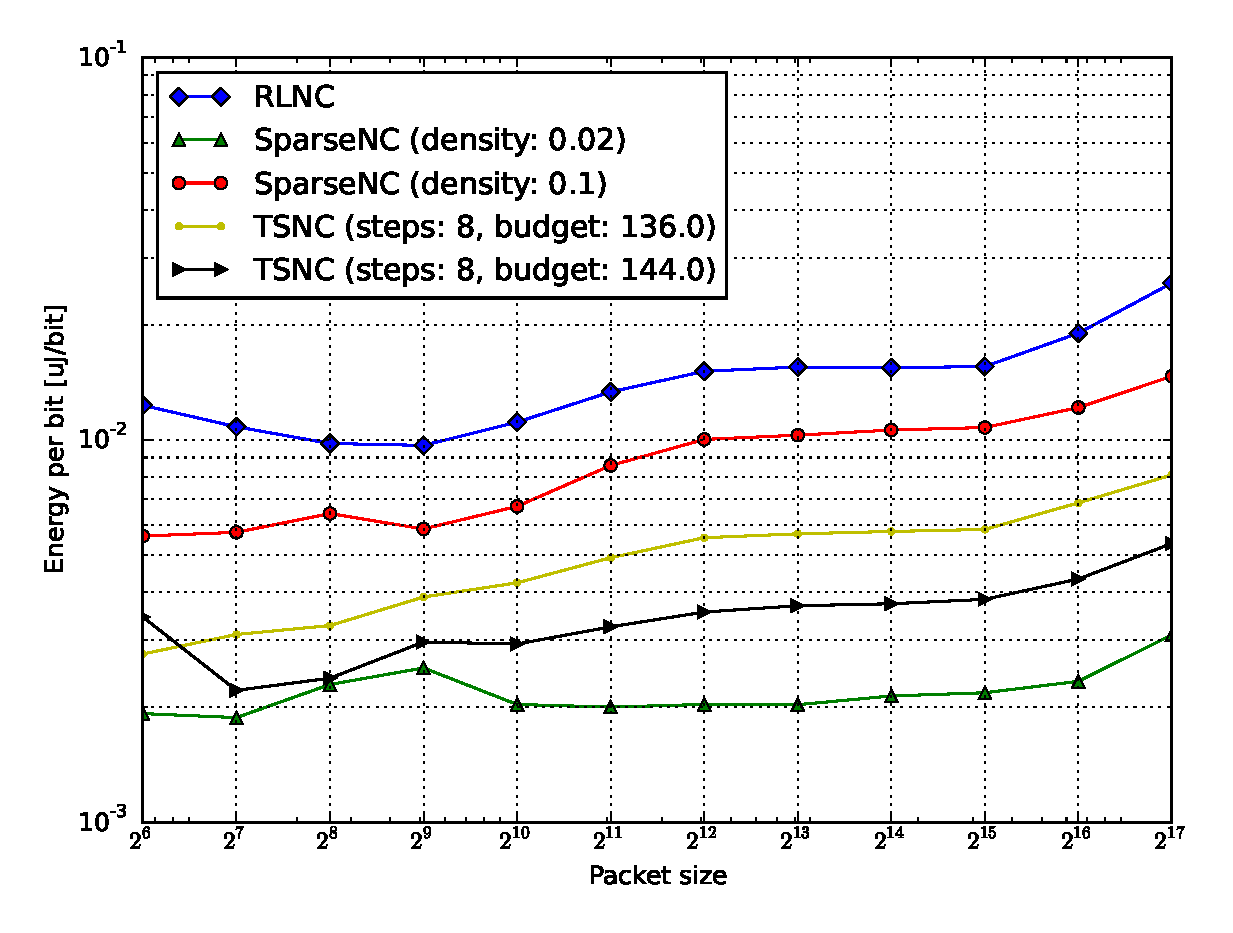
\includegraphics[width=1.1\textwidth]{images/23_07_2015/energy_per_bit_vs_symbol_size_Rasp_Binary_decoder_128.eps}
        \caption[]%
        {{\small Energy per bit vs. Packet size for $q=2,\ g=128$}}
        \label{fig:dec_ene_rasp1_packet_gf2}
    \end{subfigure}
    \quad
    \begin{subfigure}[b]{0.475\textwidth}
        \centering
        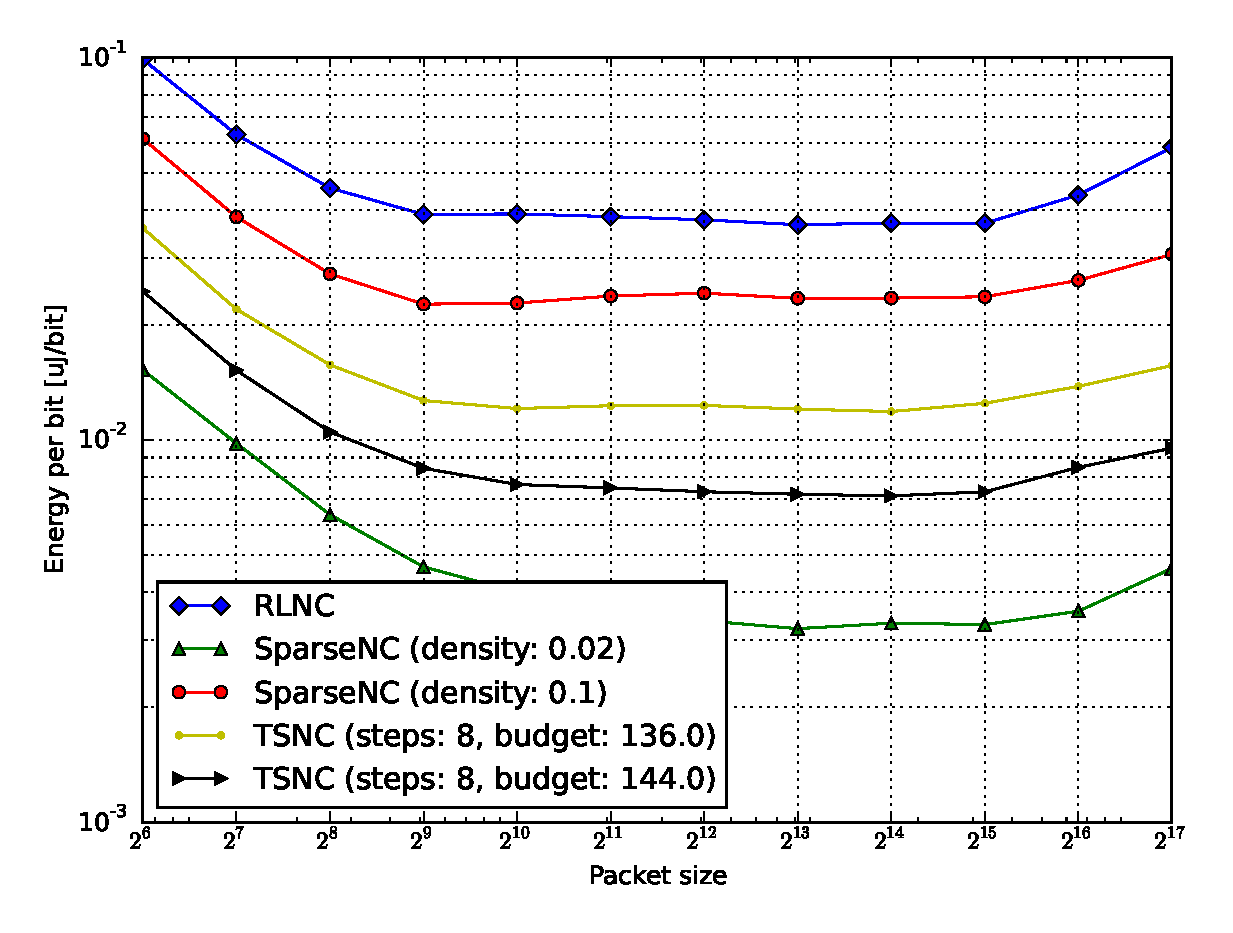
\includegraphics[width=1.1\textwidth]{images/23_07_2015/energy_per_bit_vs_symbol_size_Rasp_Binary8_decoder_128.eps}
        \caption[]%
        {{\small Energy per bit vs. Packet size for $q=2^8,\ g=128$}}
        \label{fig:dec_ene_rasp1_packet_gf256}
    \end{subfigure}
    \caption[]
    {\small Decoder energy measurements for the \ac{Raspi} 1}
    \label{fig:dec_ene_rasp1}
\end{figure*}

Raspi 2 decoding

\begin{figure*}
    \centering
    \begin{subfigure}[b]{0.475\textwidth}
        \centering
        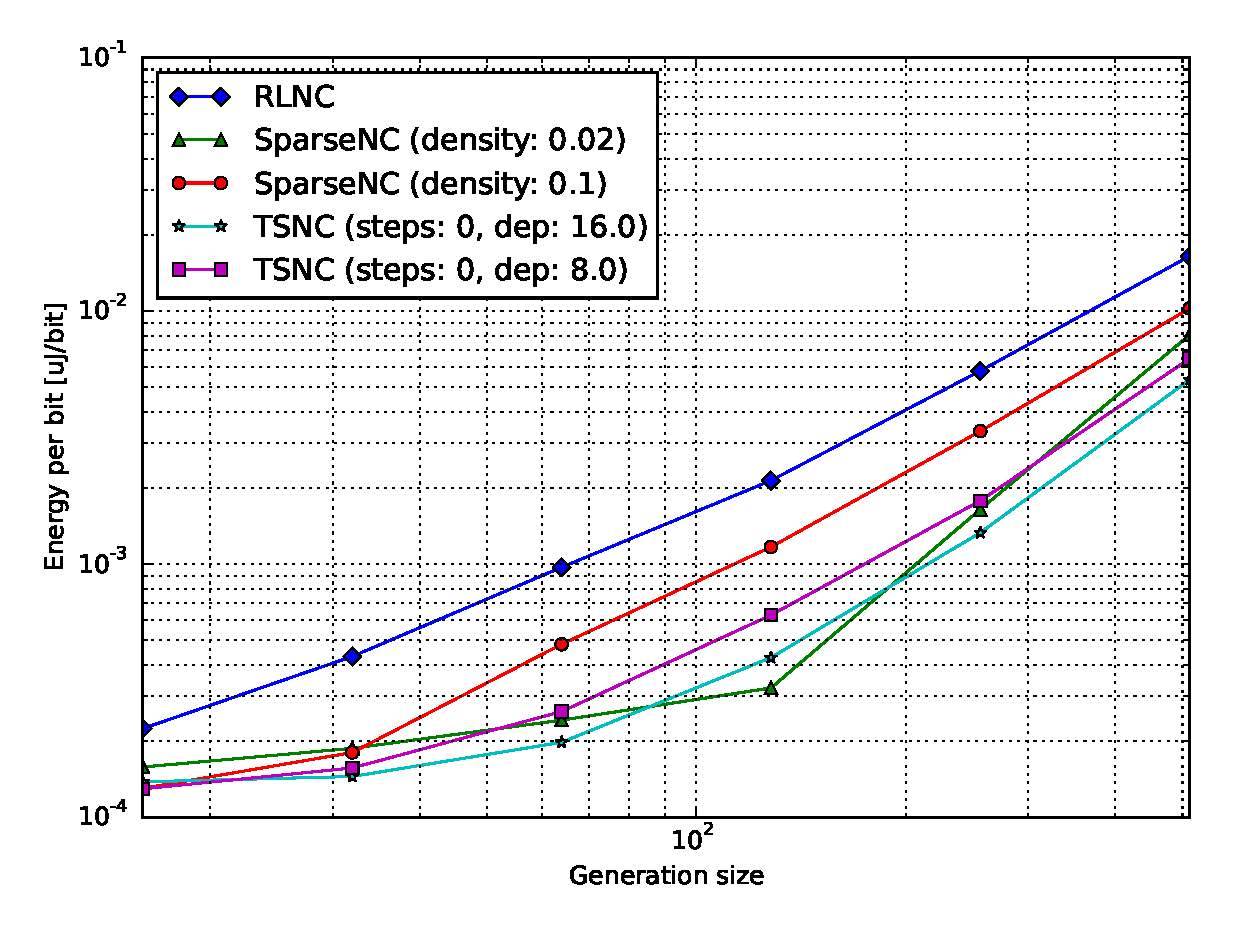
\includegraphics[width=1.1\textwidth]{images/23_07_2015/energy_per_bit_vs_generation_size_Rasp_v2_Binary_decoder_1600.eps}
        \caption[]%
        {{\small Energy per bit vs. Generation size for $q = 2$}}
        \label{fig:dec_ene_rasp2_gen_gf2}
    \end{subfigure}
    \hfill
    \begin{subfigure}[b]{0.475\textwidth}
        \centering
        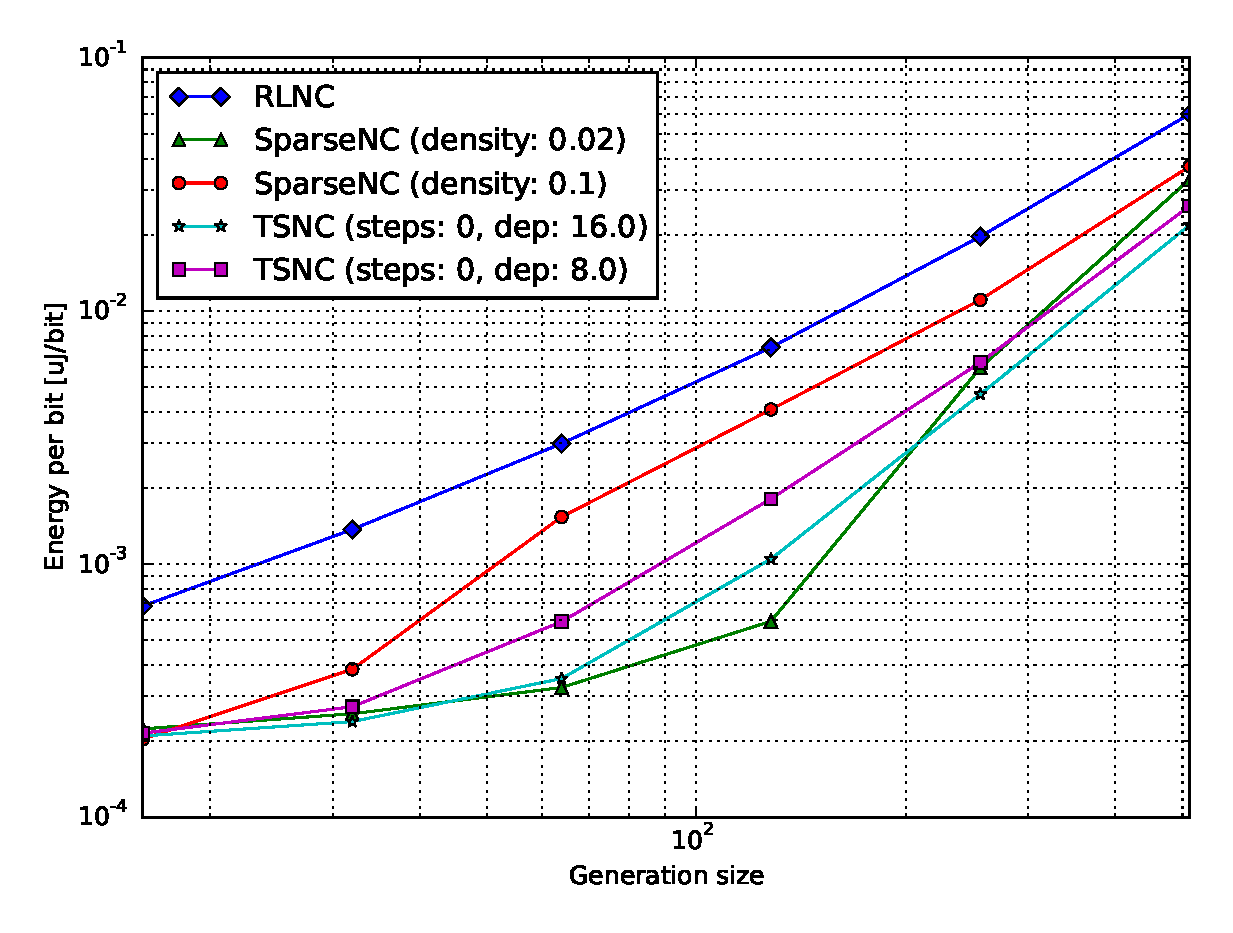
\includegraphics[width=1.1\textwidth]{images/23_07_2015/energy_per_bit_vs_generation_size_Rasp_v2_Binary8_decoder_1600.eps}
        \caption[]%
        {{\small Energy per bit vs. Generation size for $q = 2^8$}}
        \label{fig:dec_ene_rasp2_gen_gf256}
    \end{subfigure}
    \vskip\baselineskip
    \begin{subfigure}[b]{0.475\textwidth}
        \centering
        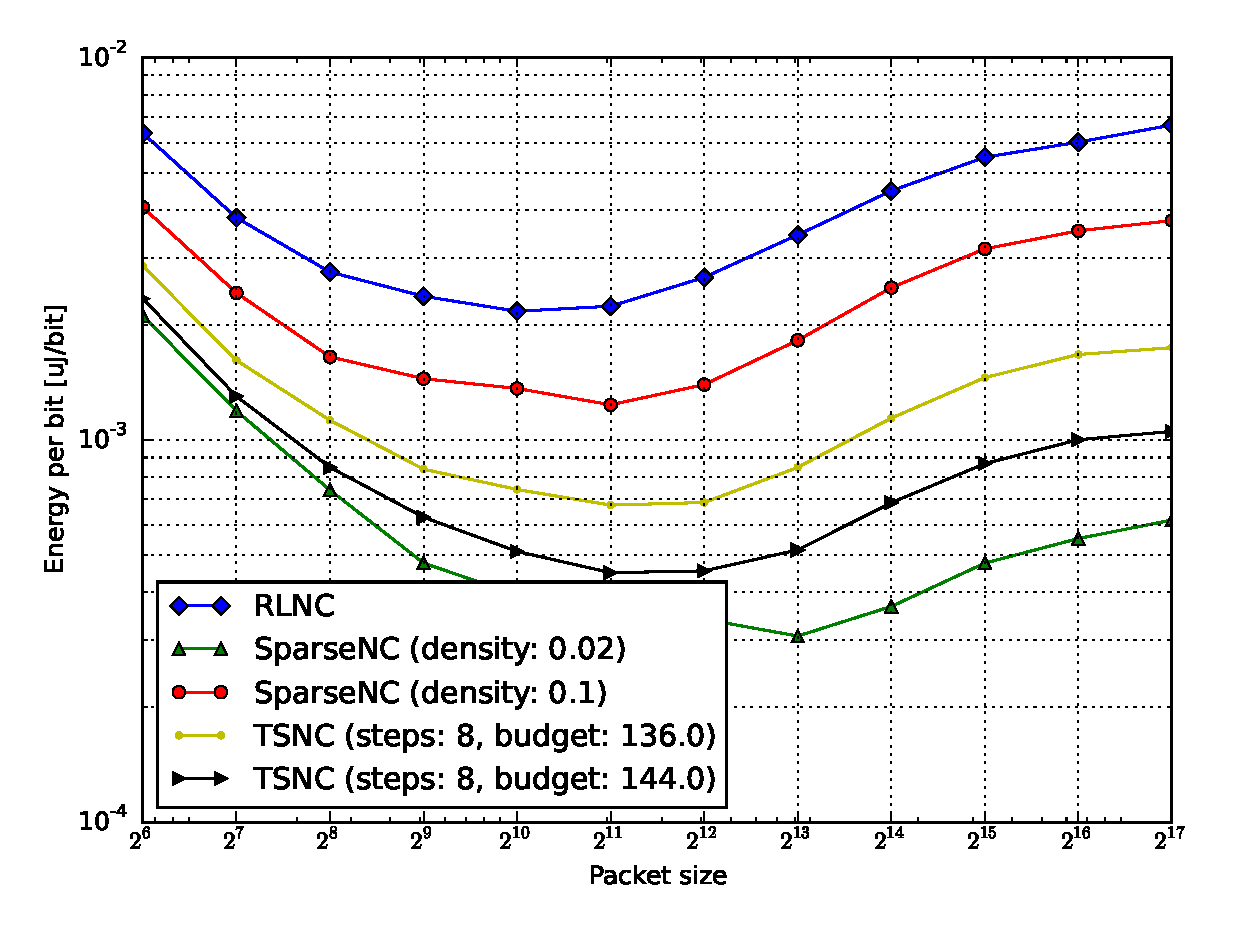
\includegraphics[width=1.1\textwidth]{images/23_07_2015/energy_per_bit_vs_symbol_size_Rasp_v2_Binary_decoder_128.eps}
        \caption[]%
        {{\small Energy per bit vs. Packet size for $q=2,\ g=128$}}
        \label{fig:dec_ene_rasp2_packet_gf2}
    \end{subfigure}
    \quad
    \begin{subfigure}[b]{0.475\textwidth}
        \centering
        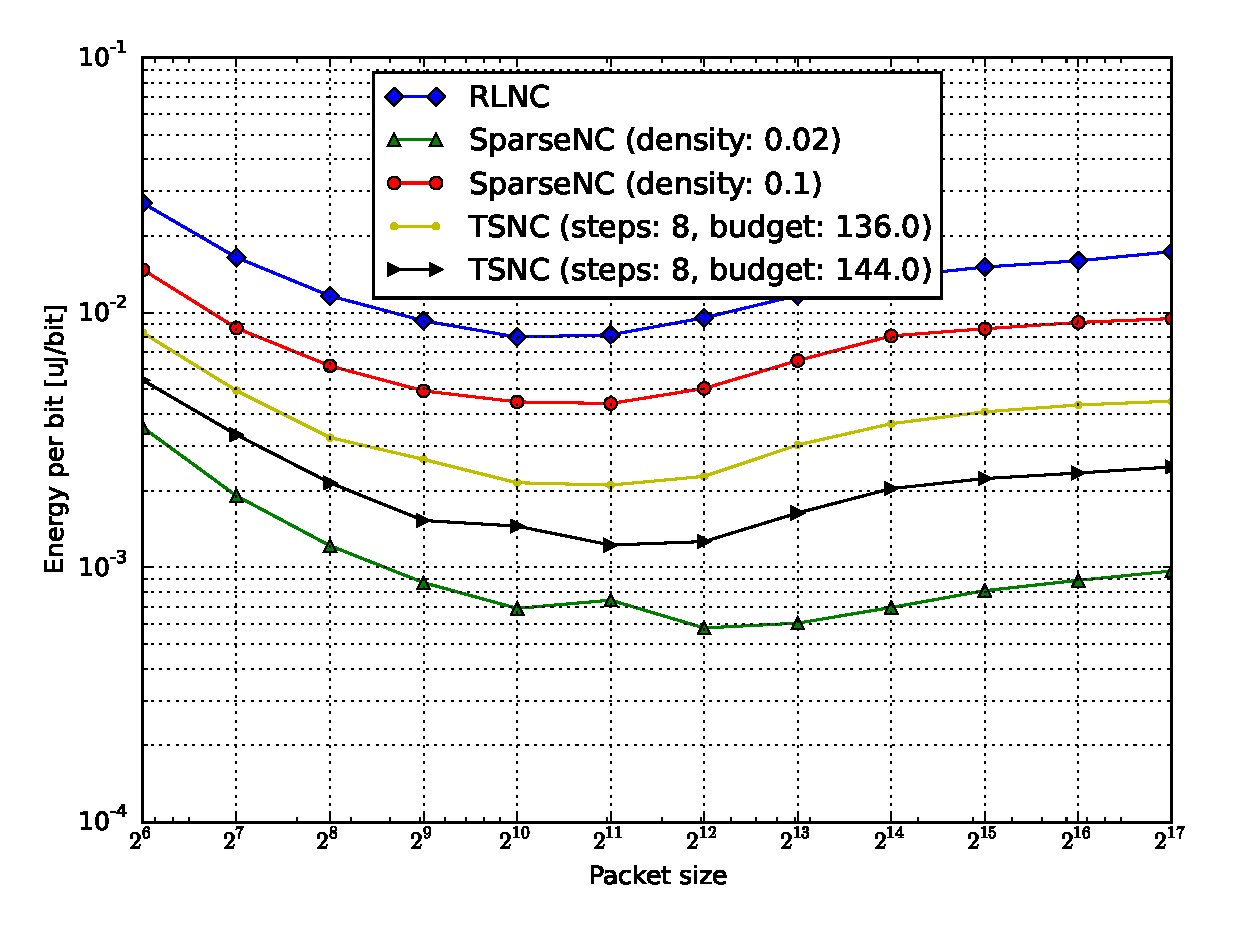
\includegraphics[width=1.1\textwidth]{images/23_07_2015/energy_per_bit_vs_symbol_size_Rasp_v2_Binary8_decoder_128.eps}
        \caption[]%
        {{\small Energy per bit vs. Packet size for $q=2^8,\ g=128$}}
        \label{fig:dec_ene_rasp2_packet_gf256}
    \end{subfigure}
    \caption[]
    {\small Decoder energy measurements for the \ac{Raspi} 2}
    \label{fig:dec_ene_rasp2}
\end{figure*}

\subsection{Multicore Network Coding}
\label{subs:multicore-network-coding}

The authors implemented the algorithm described in
Section~\ref{sub:implementation-multicore} on the Raspberry Pi 2 Model B,
which features four ARM Cortex-A7 cores in a Broadcom BCM2836 \ac{SOC}
with a 900 MHz clock. Each core has a 32 KiB L1 data cache and 32 KiB
L1 instruction cache. The cores share a 512 KiB L2 cache. All the
measured results, including the baseline results, were obtained with
NEON-enabled code adopted from the Fifi library [\textbf{Fifi reference}].
The NEON extension provides an 128-bit \ac{SIMD} instruction set to the
\ac{Raspi} 2. Figures~\ref{enc_dec1024}, \ref{enc_dec128} and
\ref{enc_dec16} show the encoding and decoding throughput in MiB per
second for different generation sizes ($g$ = 1024, 128, and 16
respectively). The throughput is the rate of generating $g$ coded packets,
divided by the time the encoder took to perform the task. The size of
each coded packet was fixed to $1536$~bytes since that is the typical
size of an Ethernet frame. The blocked operations were performed dividing
the matrices in squared sub-blocks of $16,\ 32\ ,\ 64,\ldots,\ 1024$ operands
(words in the finite field) in height and width. The figures show only
block sizes of $16 \times 16$ or $32 \times 32$ operands since with bigger
block sizes, the operands do not fit in L1 cache.

The following test cases were considered:

\subsubsection{Baseline encoding}
The baseline results involve no recording of the
\ac{DAG} and are performed in a \emph{by-the-book} fashion. The encoder uses
only one thread. And the difference between the non-blocked and blocked
encoding schemes is that in the blocked scheme, the matrix multiplications are
performed dividing the matrices in sub-blocks in order to make the algorithm
cache efficient as described in Section~\ref{sub:implementation-multicore}.

\subsubsection{Encoding blocked}
The encoding results were performed using the
method described in Section~\ref{sub:implementation-multicore}. The time
recorded includes the dependencies resolving, creation of the \ac{DAG},
and the task scheduling. In practice, it would suffice to calculate and
store this information only once per generation size.

\subsubsection{Decoding blocked}
The differences between encoding and decoding, is that the decoding task
also involves the matrix inversion. Similarly as with the encoding results,
the time recorded includes the dependencies resolving, the creation of the
\ac{DAG} and the task scheduling. However, to decode, these calculations are also made for inverting the matrix of coding coefficients.

\begin{figure}[ht!]
\centering
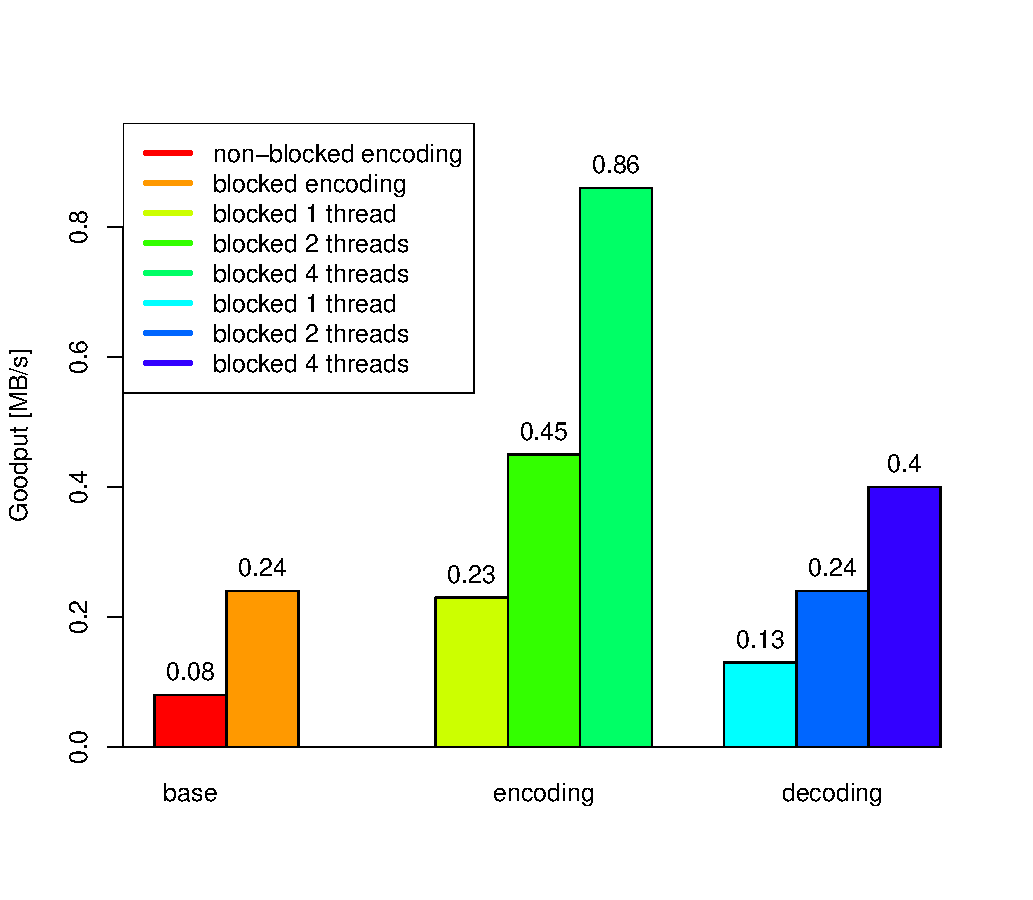
\includegraphics[width=0.7\textwidth]{images/2015-04-18_encoding_decoding_1024.pdf}
\caption{Encoding and Decoding performance for g = 1024 \cite{wunderlich2015network}}
\label{enc_dec1024}
\end{figure}

For $g=$ 1024, the blocked baseline measurements outperforms the non blocked
variant. This means that making the matrix multiplication algorithm cache
efficient brings an increase in throughput by a factor of 2.83. When using the
algorithm described in Section~\ref{sub:implementation-multicore},
encoding with four cores is on average 3.7 times faster than with one core.
Similarly, decoding with four codes is 3.05 times faster, on average, than
decoding with a single core. Figure~\ref{enc_dec1024} shows that the
implemented algorithm, by exploiting cache efficiency and only three extra
cores provides a gain of 10 folds compared with traditional non-blocked
algorithms. With $g$ = 1024, the matrix inversion becomes more expensive
than at smaller generations sizes. Therefore, the decoding throughput
is 46\% of the encoding throughput.

\begin{figure}[ht!]
\centering
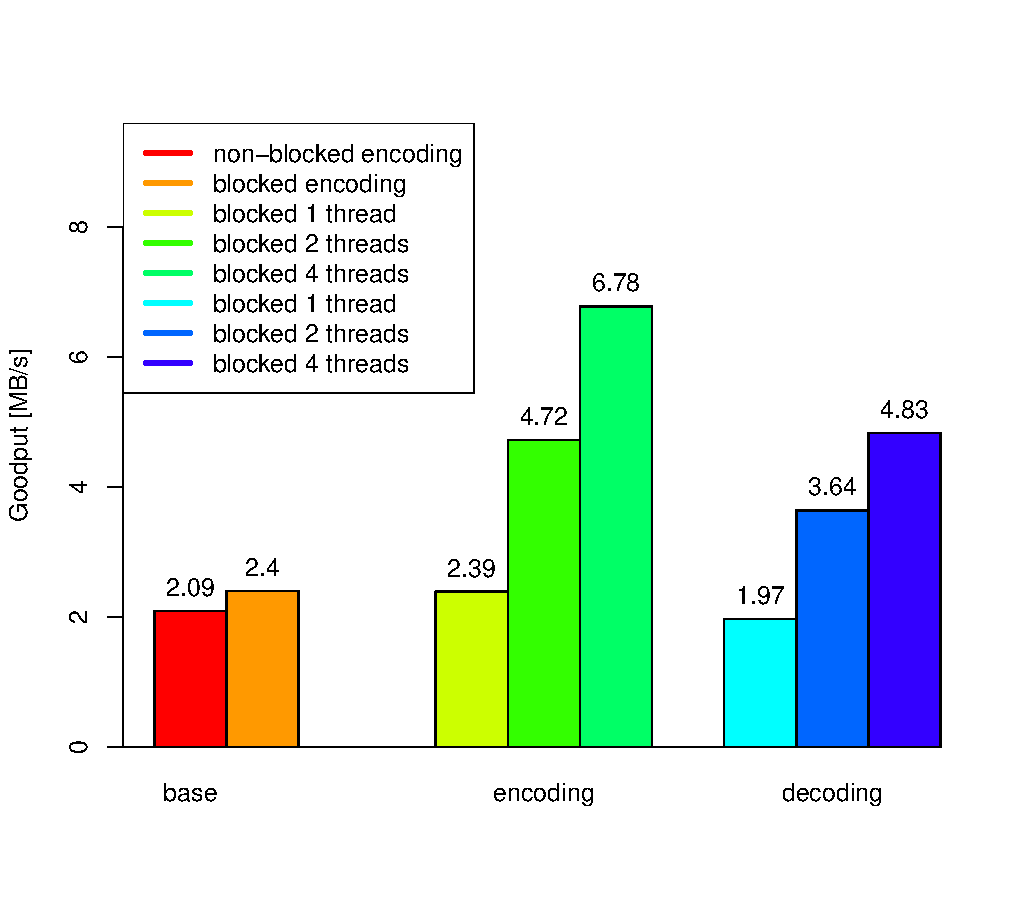
\includegraphics[width=0.7\textwidth]{images/2015-04-18_encoding_decoding_128.pdf}
\caption{Encoding and Decoding performance for g = 128 \cite{wunderlich2015network}}
\label{enc_dec128}
\end{figure}

For $g$ = 128, the differences between the baselines operations show that a
blocked algorithm is 15\% faster than the non-blocked variant. Encoding with
four cores is 2.82 times faster than with a single core. Due to the smaller
matrix sizes, the gain when using blocked operations in the baselines is not
that significant when compared with $g$ = 1024. For the same reason, the matrix
inversion is less expensive. As a consequence, the decoding throughput is 71\%
of the encoding throughput.

\begin{figure}[ht!]
\centering
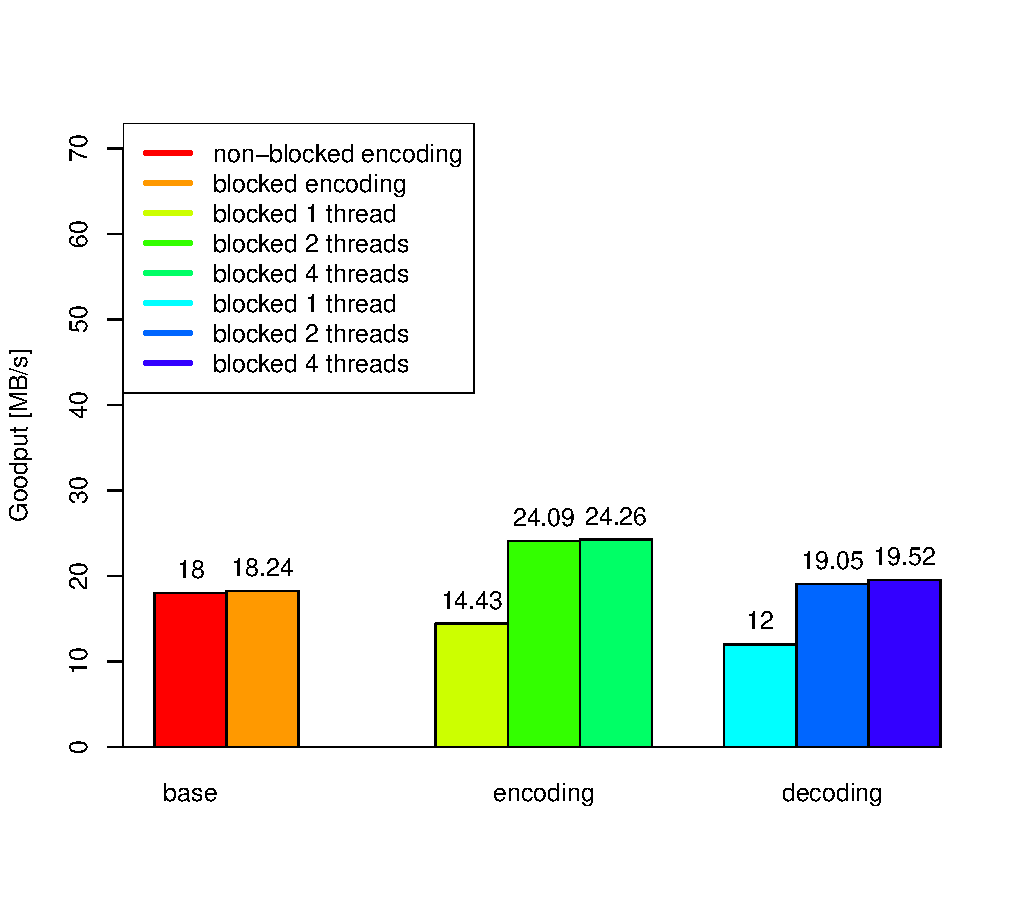
\includegraphics[width=0.7\textwidth]{images/2015-04-18_encoding_decoding_16.pdf}
\caption{Encoding and Decoding performance for g = 16 \cite{wunderlich2015network}}
\label{enc_dec16}
\end{figure}

When $g$ = 16, the gains of blocked operations are negligible compared with
the non-blocked ones. The reason behind this behavior is that all the data
fits in the L1 cache. For the scheduled version, since the problem to solve
is so small, the gain when using four cores is a factor of 1.68 compared
with a single core, and 1.01 compared with two cores. Therefore, there
are no practical benefits in using four cores instead of two.

The differences in throughput, for all generation sizes, between the
blocked baseline and the single threaded scheduled measurements are due the
time spent resolving the dependencies and the scheduling overhead. These
effects are negligible for big generation sizes, while considerable for
small matrices.

\subsubsection{Comparison of the load of matrix multiplications and inversions}

To compare how much slower is the matrix multiplication with respect to the
matrix inversion for different generation sizes, we ran a set of tests. We used
a single core to perform the operations. We changed the generation sizes,
performed matrices multiplications and matrix inversions, and measured the time
spent doing so which we name $T_{mult}$ and $T_{inv}$. We calculate the ratio
between these two measured times defined as $r = \frac{T_{mult}}{T_{inv}}$.
Table~\ref{runtimes} summarizes the results. The bigger the matrix size, the
smaller is the calculated ratio. This means that when the problems are bigger,
the decoding throughput decreases compared with the encoding throughput.

\begin{table}[H]
\center
\caption{Multiplication and inversion run-times for different generation sizes with 1 thread}
\begin{tabular}{|r|r|r|r|}

\hline
$g$ & $T_{mult}$ (ms) & $T_{inv}$ (ms) &$r$ \\
\hline
\hline

	16   & 1.703     & 0.345    & 4.9 \\
\hline
	32   & 6.573     & 0.914    & 7.2 \\
\hline
	64   & 21.341    & 3.479    & 6.1 \\
\hline
	128  & 82.326    & 17.411   & 4.7 \\
\hline
	256  & 336.398   & 106.861  & 3.1 \\
\hline
	512  & 1548.750  & 659.469  & 2.3 \\
\hline
	1024 & 6730.380  & 5166.920 & 1.3 \\
\hline
\end{tabular}
\vspace{0.2cm}
\label{runtimes}
\end{table}
